\documentclass[a4j,12pt]{jreport}

% 図を利用する場合
\usepackage{url}

\usepackage{amsmath}
\usepackage{amssymb}


%表のセル内で改行する場合
\usepackage{multirow}

%SI単位を利用する場合
\usepackage{siunitx}

\usepackage[dvipdfmx]{graphicx}

\usepackage{comment}
\usepackage {threeparttable}

\usepackage{listings,plistings}
\usepackage{graphicx}
\usepackage{here}
\usepackage[top=25truemm,bottom=25truemm,left=25truemm,right=25truemm]{geometry}

\usepackage{otf}
\usepackage{ulem}

\usepackage[hang,small,bf]{caption}
\usepackage[subrefformat=parens]{subcaption}

%% カラムサイズの指定用 %%
\newcolumntype{C}[1]{>{\centering\arraybackslash}p{#1}}
\newcolumntype{L}[1]{>{\raggedright\arraybackslash}p{#1}}
\newcolumntype{R}[1]{>{\raggedleft\arraybackslash}p{#1}}

%% 上下中央揃え%%
\newcommand{\CenterRow}[2]{
  \dimen0=\ht\strutbox%
  \advance\dimen0\dp\strutbox%
  \multiply\dimen0 by#1%
  \divide\dimen0 by2%
  \advance\dimen0 by-.5\normalbaselineskip%
  \raisebox{-\dimen0}[0pt][0pt]{#2}}

\captionsetup{compatibility=false}

\begin{document}

\setcounter{tocdepth}{6}
\setcounter{secnumdepth}{6}

\thispagestyle{empty}

\vspace*{2cm}
\begin{center}

{\LARGE ああああ}\vfill
\vspace*{7cm}
{\LARGE 22RS012}\vfill
{\huge 井上 誠斗}

\vspace*{20mm}
{\LARGE 九州産業大学 理工学部}\vfill
{\LARGE 情報科学科}\vfill

\vspace*{20mm}
{\LARGE 令和8年 1月}
\vfill
\end{center}


%\thispagestyle{empty}
%{\par \baselineskip=.8\normalbaselineskip
%\begin{quotation}
%\pagenumbering{roman}\setcounter{page}{0}
%\tableofcontents
%\listoffigures
%\listoftables\vfill
%\end{quotation} \par}
%\vskip  \textwidth \pagebreak
%\setcounter{page}{1}\pagenumbering{arabic}
%\renewcommand{\bibname}{参考文献}



%%%%%%%%%%%%%%%%%%%%%%%%%%%%%%%%%%%%%%%%%%%%%%
\chapter{序論}\label{chap:Introduction}
%序論


\section{研究背景}

2019年末に中国武漢市で報告された新型コロナウイルス感染症(COVID-19)は,短期間のうちに世界的な流行へと発展し,2020年以降の日常生活,教育,産業活動に深刻な影響を及ぼした.各国において外出制限や行動制限が実施され,人々の生活様式は大きく変化した.COVID-19 は飛沫感染に加え,微小な粒子であるエアロゾルを介した空気感染の可能性が指摘されており,特に換気が不十分な室内環境では感染リスクが著しく高まることが明らかになっている.この状況を受け,厚生労働省は密閉・密集・密接のいわゆる「三つの密」を回避する行動を国民に呼びかけた.なかでも密閉空間における換気の重要性は,学校や職場,公共施設などあらゆる場面で強調され,空気環境への関心が社会全体で急速に高まる契機となった.

このような背景のもと,室内の換気状態を把握するための定量的な指標として CO$_2$ 濃度に注目が集まった.CO$_2$ は人体の呼気に多く含まれるため,室内における滞在人数や人の密度を間接的に反映する指標として利用できる.換気が不十分な環境では CO$_2$ 濃度が上昇しやすく,その変化を観測することで換気状態を把握することが可能である.このため,CO$_2$ 濃度の上昇は換気不足を示す重要なサインとなり,空気環境評価において有効な指標として位置付けられている.実際にコロナ禍では,学校,飲食店,公共施設など多くの場所で CO$_2$ センサの設置が進められ,数値によって換気状態を可視化する取り組みが広く実施された.これにより,CO$_2$ 濃度は感染症対策を支援する実用的な環境指標として社会に定着したといえる.

一方で,2023年以降は社会活動が徐々に平常化し,人々の行動制限や感染対策が緩和される傾向が見られるようになった.その結果,季節性インフルエンザをはじめとする呼吸器感染症が全国的に大流行する状況が続いている.特に注目すべき点として,コロナ禍にあたる2020〜2021年には,インフルエンザの報告件数が過去に例を見ないほど低水準であったことが挙げられる.この現象は,マスク着用や人流抑制といった行動変容に加え,換気の徹底が感染拡大の抑制に大きく寄与していた可能性を示唆している.すなわち,換気は COVID-19 に限らず,インフルエンザなどの広範な呼吸器感染症に対しても有効な対策であると考えられる.

以上のように,COVID-19 を契機として空気環境の重要性は社会的に広く認識されるようになったが,換気の有効性は一時的な感染症対策にとどめるべきではない.特に,教育機関,オフィス,飲食店など,多くの人が集まる空間では,平常時においても継続的な空気質管理が求められる.さらに,個人レベルにおいても,自宅,車内,店舗,移動先など多様な環境で空気質を把握できる仕組みが重要である.しかし,既存の CO$_2$ センサの多くは据え置き型であり,設置場所が限定されるという課題がある.このような背景から,柔軟に持ち運びが可能で,日常生活の中でさまざまな環境における空気質を把握できる CO$_2$ 測定機器の必要性が高まっている.

\begin{figure}[h]
\centering
\includegraphics[width=.5\linewidth]{./figures/av7et-x4rpq}
\caption{ESP32-C6}
\label{fig:mune}
\end{figure}




\section{CO$_2$濃度と空気環境}

CO$_2$濃度は,室内の空気環境を評価するための代表的な指標の一つである.大気中の主要成分のうち,CO$_2$は約 0.04\% と非常に低い割合しか占めていないが,室内空間では人の呼気によって短時間で濃度が上昇する特徴を持つ.そのため,CO$_2$濃度の変化は,室内における人の滞在状況や換気の十分さを間接的に反映する指標として広く利用されている.このような性質から,CO$_2$濃度は空気質評価において重要な役割を果たしている.

CO$_2$濃度は ppm(parts per million)を単位として表され,屋外環境では一般に 415〜450 ppm 程度でほぼ一定の値を示す.一方,換気が不十分な室内環境では,人の呼吸活動により CO$_2$濃度が急激に上昇することが知られている.このため,屋外濃度と室内濃度の差を観測することで,換気状態の良否を定量的に評価することが可能である.特に,多人数が長時間滞在する空間では,CO$_2$濃度の継続的な監視が重要となる.

CO$_2$濃度に関しては,国の指針や基準においても具体的な数値が示されている.厚生労働省の「建築物環境衛生管理基準」では,空気調和設備を備える居室において,CO$_2$濃度を 1,000 ppm 以下に維持することが求められている.また,文部科学省の「学校環境衛生基準」では,教室内の換気状態を判断する目安として 1,500 ppm 以下が望ましいとされている.これらの基準は,CO$_2$濃度が室内空気環境の良否を判断する実用的な指標であることを示している.

さらに,CO$_2$濃度の上昇は換気不良を示すだけでなく,人の健康や作業効率にも影響を及ぼすことが報告されている.具体的には,CO$_2$濃度の上昇に伴い,集中力の低下,頭痛,眠気,疲労感などの症状が現れる可能性が指摘されている.特に学習環境においては,CO$_2$濃度が 1,000 ppm を超えると児童生徒の認知機能や学習効率が低下することが示されており,教育現場における空気質管理の重要性が強調されている.

以上のように,CO$_2$濃度は換気状態を把握するための環境指標であると同時に,人の健康や快適性,作業・学習効率に直結する重要な要素である.そのため,感染症リスクの低減や快適な居住・活動環境を実現する上で,CO$_2$濃度を継続的に把握し,適切な換気を行うことが不可欠である.


\section{換気・温湿度と感染症リスク}
空気環境の指標としては CO$_2$濃度だけでなく,温度・湿度も重要である.先行研究では,低温環境や過度に乾燥した環境が呼吸器系疾患の罹患率を高めることが報告されており,適切な温湿度管理は感染症対策としても不可欠である.

COVID-19 だけでなく,インフルエンザウイルスなどの多くの呼吸器ウイルスは,乾燥した空気中で生存しやすく,また低温環境では免疫機能が低下し感染しやすくなることが知られている.さらに,換気不足の環境ではウイルスを含むエアロゾルが滞留し,同一空間内での集団感染リスクを高める.

このように,空気環境と感染症リスクは密接に関連しており,CO$_2$濃度と温湿度を総合的に把握することが,快適性の向上だけでなく,感染症予防・健康維持の観点からも重要である.
\begin{figure}[h]
\centering
\includegraphics[width=.5\linewidth]{./figures/av7et-x4rpq}
\caption{ESP32-C6}
\label{fig:mune}
\end{figure}




\section{現在の課題}
近年,COVID-19 を契機として室内の換気状況を可視化する手段として CO$_2$ センサの普及が急速に進んだ.しかし,現在広く利用されている多くの CO$_2$ 測定機器には,使用環境や対象に応じていくつかの課題が残されている.

第一に,既存の CO$_2$ センサの多くは据え置き型として設計されており,設置位置により測定結果が大きく変動するという問題がある.室内環境は空気の流れや空間の形状,人の動きに大きく影響されるため,換気の不十分な場所とそうでない場所が混在することがある.したがって,一台の据え置き型センサでは空間全体の換気状況を把握することが困難であり,複数台のセンサを導入する必要が生じる.しかし,複数台を設置するためにはコストや設置場所の確保といった制約があり,特に個人利用や小規模環境においては現実的ではない.

第二に,既存製品はサイズが大きく携帯性に乏しいため,利用者が自宅,大学,飲食店,車内など複数の環境を移動しながら空気質を測定するといった使い方には適していない.実際には,密閉空間や混雑した空間に入る前に換気状態を確認したい場面は日常的に多く存在するが,現状の測定器はそのような用途に十分に応えられていない.

第三に,精度の高い NDIR 式 CO$_2$ センサは価格が高く,一般利用者が複数の環境で使用するには導入コストが大きな負担となる.またセンサの精度が高くても,消費電力が大きくバッテリ駆動に向かない製品も多いため,携帯型デバイスとして長時間使用することが難しいという課題がある.

さらに,COVID-19 の流行以降,換気の重要性は社会的に広く認識されるようになった一方,2023 年以降の社会活動の再開に伴ってインフルエンザの大規模な流行が再び発生している.この状況は,感染症対策としての空気環境管理が依然として必要であることを示しているが,現状では個々人が自らの生活環境における換気状態を能動的に把握し,適切な判断を行うための手軽なツールが不足している.

以上のように,据え置き型 CO$_2$ センサでは測定場所が限定されること,小型で携帯性に優れた測定機器が不足していること,そして個人が移動先の空気環境を評価する手段が十分に整備されていないことなど,現行の環境計測機器には依然として多くの課題が存在する.

\begin{figure}[h]
\centering
\includegraphics[width=.5\linewidth]{./figures/av7et-x4rpq}
\caption{ESP32-C6}
\label{fig:mune}
\end{figure}


\section{本研究の目的}
本研究の目的は,従来の据え置き型 CO$_2$ センサの課題を踏まえ,携帯可能でありながら高精度な測定が可能な小型 CO$_2$ 測定デバイスを試作し,日常生活における多様な環境での空気質把握を可能にすることである.

具体的には,センサシステム全体の小型化・省電力化を図り,モバイルバッテリや内蔵電源によって長時間稼働できる CO$_2$ 測定デバイスの実現を目指す.これにより,自宅や大学といった固定的な環境だけでなく,車内,カフェ,研究室,イベント会場など,利用者が移動しながら直面するさまざまな環境の換気状況を簡便に評価できるようにする.また,NDIR 方式を採用した高精度な CO$_2$ 測定を可能とし,空気質の変化をリアルタイムで取得できるように設計することで,換気の不足を素早く検知し,感染症予防や健康維持につながる判断を支援する.

本研究では,試作した小型 CO$_2$ 測定デバイスを複数の環境で実際に使用し,CO$_2$ 濃度の変動や換気状態の違いを測定・評価する.これにより,デバイスの実用性や測定精度,省電力性能を検証し,持ち運び型空気質モニタとしての有効性を明らかにすることを目指す.さらに,測定結果を通じて,空気質の改善や適切な換気行動を促すための新たな知見を得ることも期待される.

以上の取り組みにより,個人が日常生活の中で空気環境に対する意識を高め,安全で快適な生活空間を維持するための一助となる測定デバイスの開発を目指す.

%%%%%%%%%%%%%%%%%%%%%%%%%%%%%%%%%%%%%%%%%%%%%%
\chapter{開発環境}\label{chap:development}
% 開発環境


%%%%%%%%%%%%%%%%%%%%%%%%%%%%%%%%%%%%%%%%%%%%%%%%

\section{概要}
本章では,本研究において使用した開発環境および機器について述べる。
本研究では,新規に試作した携帯型CO$_2$測定デバイスを中心に,マイクロコントローラ,センサ,通信モジュール,電源系を含むハードウェア構成を設計・実装した。
また,性能比較および有効性検証のため,先行研究で使用された機器についても併せて説明する。

\section{新規に作成した機器}
本研究では,携帯型CO$_2$測定デバイスの実現を目的として,新たにハードウェア構成を設計・試作した。
本節では,試作機を構成する各機器について説明する。

\subsection{マイクロコントローラ ESP32-C6}
本研究では,マイクロコントローラとして Seeed Studio XIAO ESP32-C6 を採用した。
本モジュールは ESP32-C6 SoC を搭載しており,2つの32ビット RISC-V プロセッサで構成されている。
高性能(High Performance: HP)プロセッサは最大160\,MHzで動作し,低消費電力(Low Power: LP)プロセッサは最大20\,MHzでの動作が可能である。

また,512\,KBのSRAMおよび4\,MBのフラッシュメモリを内蔵しており,センサ制御,通信処理,データ管理を同時に行うIoT用途に十分な記憶容量を備えている。
無線通信機能として,2.4\,GHz Wi-Fi 6,Bluetooth 5.3,Zigbee,Thread(IEEE 802.15.4)をサポートしており,Matterにネイティブ対応している点も特徴である。

これらの特性から,本研究では高い演算性能と低消費電力動作を両立できるマイクロコントローラとして ESP32-C6 を採用した。

\begin{figure}[H]
\centering

\begin{minipage}{0.42\linewidth}
  \centering
  \includegraphics[width=\linewidth]{./figures/SeeedESP32C6}
  \captionof{figure}{SeeedESP32C6}
  \label{fig:SeeedESP32C6}
\end{minipage}
\hfill
\begin{minipage}{0.52\linewidth}
  \centering
  \captionof{table}{ESP32C6の主なパラメータ}
  \label{tab:scd41Parameters}
  \begin{tabular}{|c|c|}
    \hline
    モデルNo. & SCD41 \\ \hline \hline
    I2Cアドレス & 0x62 \\ \hline
    測定対象 & CO$_2$,温度,湿度 \\ \hline
    CO$_2$測定範囲 & 400$\sim$5000 ppm \\ \hline
    CO$_2$測定精度 & $\pm$(40 ppm + 5\%) \\ \hline
    温度測定範囲 & -10$\sim$60 ℃ \\ \hline
    湿度測定範囲 & 0$\sim$95 \%RH \\ \hline
    解像度 & 16ビット \\ \hline
    入力電圧 & 2.4$\sim$5.5 V \\ \hline
    平均消費電流 & 約15 mA \\ \hline
    ボード寸法 & 約10.1 $\times$ 10.1 $\times$ 7.0 mm \\ \hline
    対応温度 & -10$\sim$60 ℃ \\ \hline
  \end{tabular}
\end{minipage}

\end{figure}


\FloatBarrier


\subsection{CO$_2$センサモジュール SCD41}
二酸化炭素濃度は,室内空気質を評価する上で重要な指標の一つであり,換気状態や居住環境の快適性と密接に関係している。
本研究では,CO$_2$センサとして Sensirion 社製 SCD41 を搭載したモジュールを使用した。

SCD41 は NDIR(Non-Dispersive Infrared)方式を採用した高精度なCO$_2$センサであり,小型かつ低消費電力である点が特徴である。
また,温度および湿度センサを内蔵しており,これらの測定値を用いた補正により,安定したCO$_2$濃度測定が可能である。

本モジュールは 2.54\,mm ピッチのピンインターフェースを備えており,I$^2$C通信によってマイクロコントローラと接続される。
これにより,携帯型デバイスへの組み込みが容易であり,本研究の目的に適している。
本モジュールの主なパラメータを表\ref{tab:scd41Parameters}に示す。


\begin{figure}[H]
\centering

\begin{minipage}{0.42\linewidth}
  \centering
  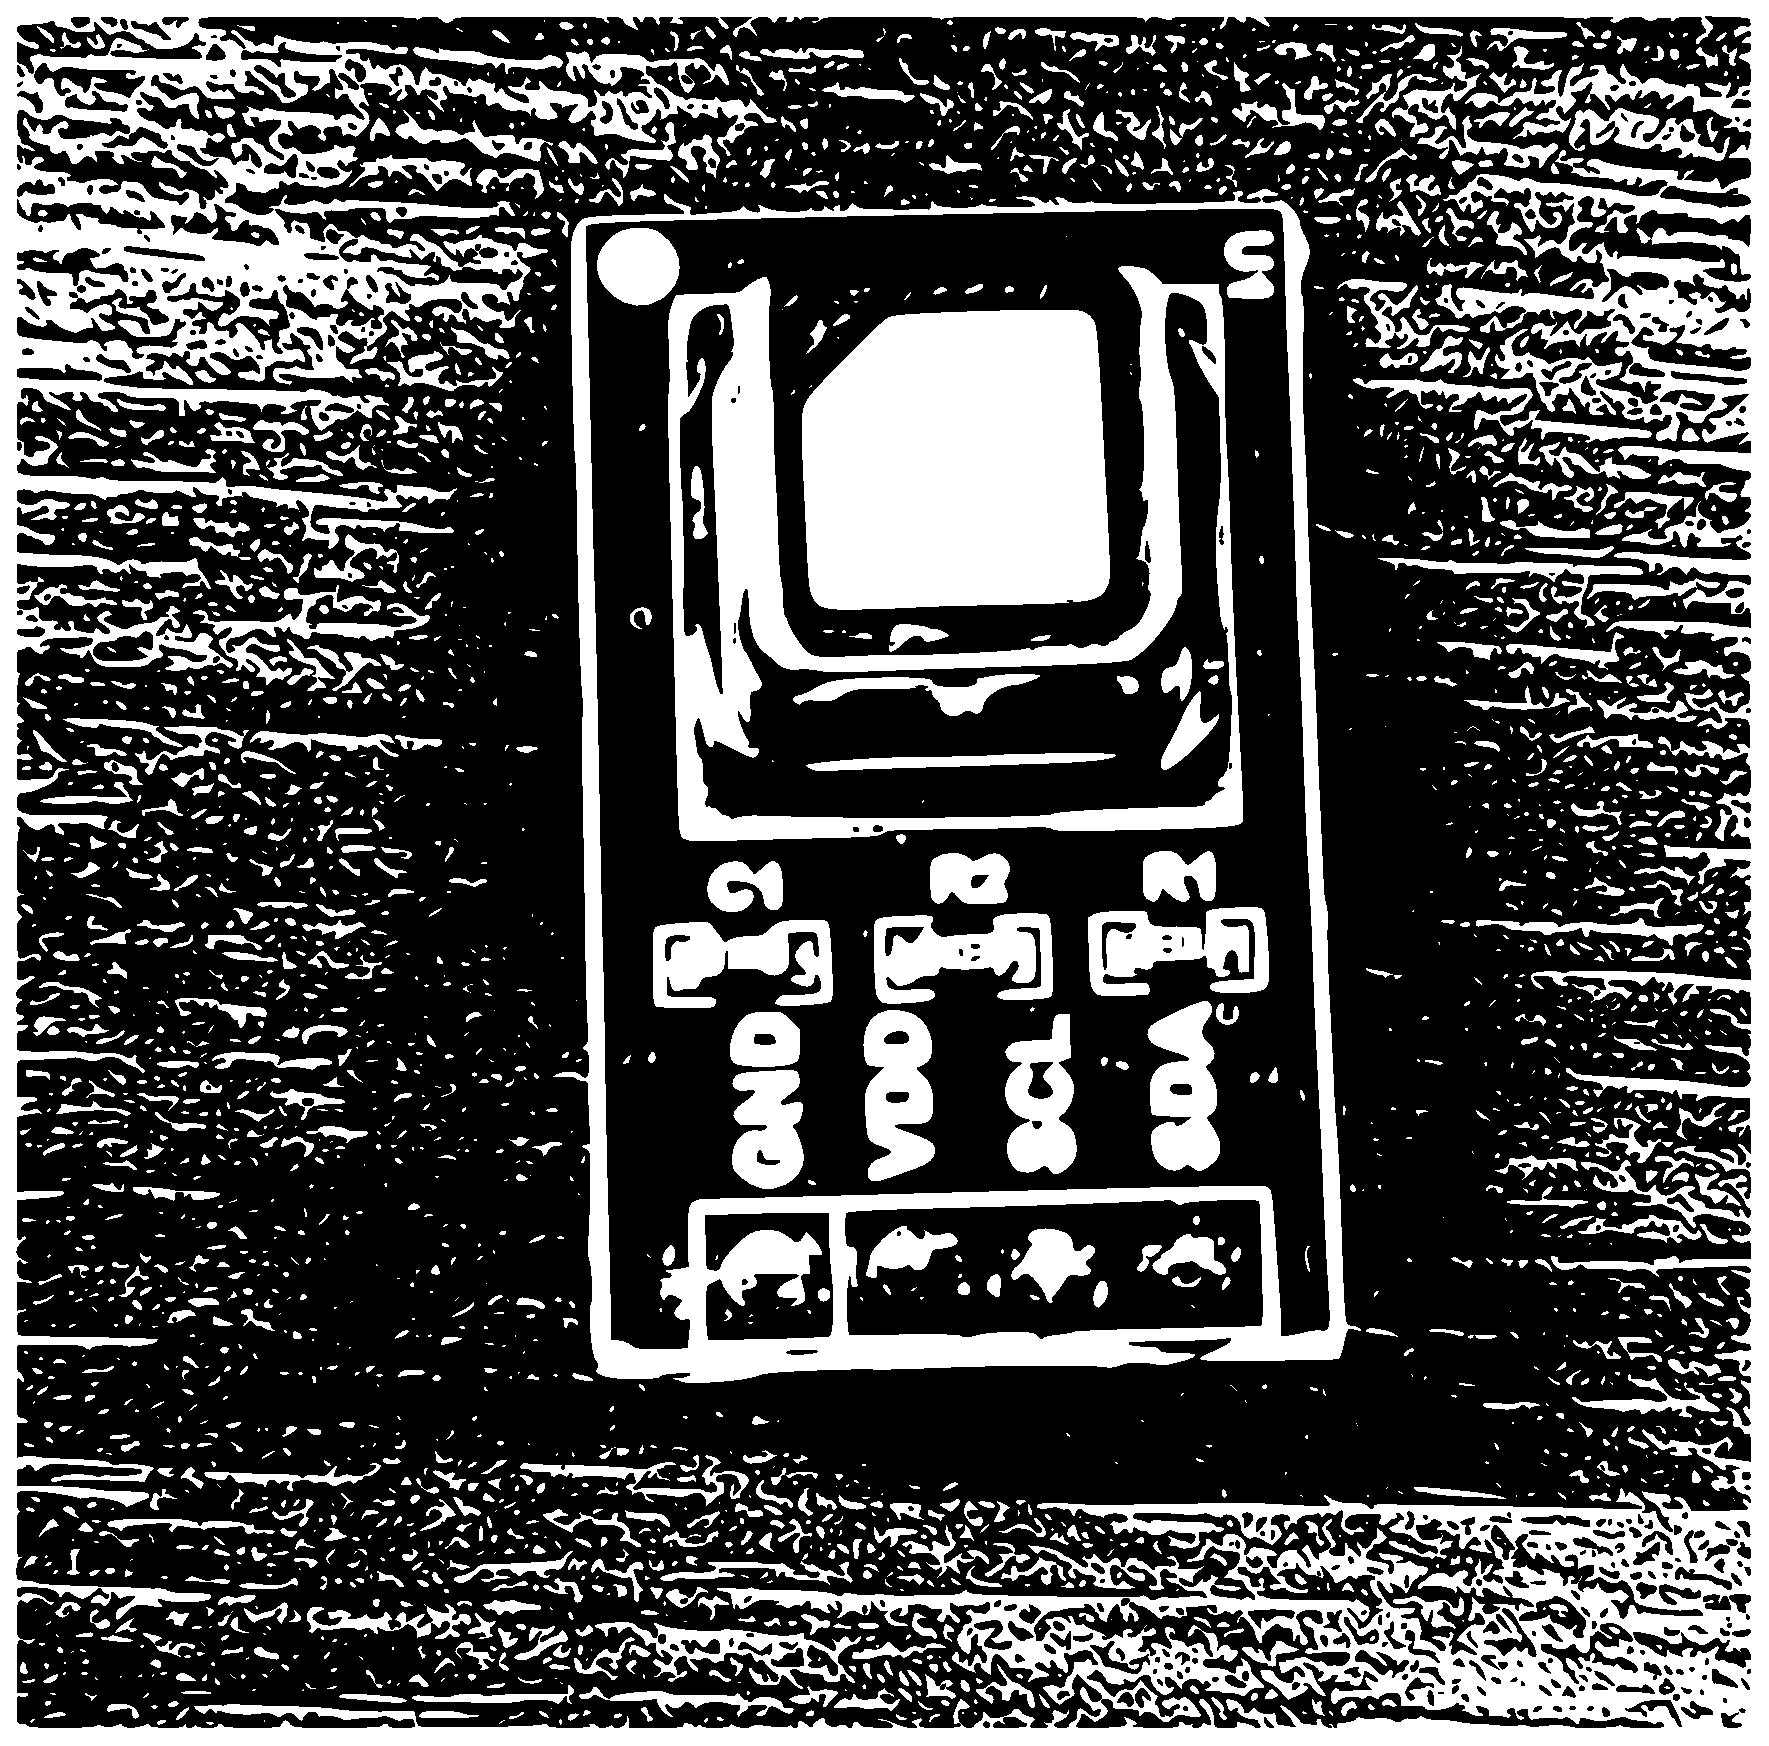
\includegraphics[width=\linewidth]{./figures/scd41_new}
  \captionof{figure}{SCD41}
  \label{fig:sensor}
\end{minipage}
\hfill
\begin{minipage}{0.52\linewidth}
  \centering
  \captionof{table}{SCD41の主なパラメータ}
  \label{tab:scd41Parameters}
  \begin{tabular}{|c|c|}
    \hline
    モデルNo. & SCD41 \\ \hline \hline
    I2Cアドレス & 0x62 \\ \hline
    測定対象 & CO$_2$,温度,湿度 \\ \hline
    CO$_2$測定範囲 & 400$\sim$5000 ppm \\ \hline
    CO$_2$測定精度 & $\pm$(40 ppm + 5\%) \\ \hline
    温度測定範囲 & -10$\sim$60 ℃ \\ \hline
    湿度測定範囲 & 0$\sim$95 \%RH \\ \hline
    解像度 & 16ビット \\ \hline
    入力電圧 & 2.4$\sim$5.5 V \\ \hline
    平均消費電流 & 約15 mA \\ \hline
    ボード寸法 & 約10.1 $\times$ 10.1 $\times$ 7.0 mm \\ \hline
    対応温度 & -10$\sim$60 ℃ \\ \hline
  \end{tabular}
\end{minipage}

\end{figure}

\FloatBarrier

\subsection{リチウムポリマバッテリ}
本研究で試作した携帯型CO$_2$測定デバイスの電源として,リチウムポリマバッテリを使用した。
リチウムポリマバッテリは,高エネルギー密度,小型・軽量である点から,携帯機器やウェアラブルデバイスに広く利用されている。

本研究では,長時間駆動および携帯性の両立を目的として,バッテリ駆動による動作を前提とした設計を行った。

\subsection{LTE通信モジュール SIM7080G}
通信モジュールとして,SIMCom 社製 SIM7080G を使用した。
SIM7080G は,LTE Cat.M1 および NB-IoT に対応した低消費電力通信モジュールであり,M2M および IoT 用途に特化して設計されている。

本モジュールは Qualcomm 製コアを搭載し,省電力クラス Class~5 に対応している。
また,グローバルモデルであるため,幅広い通信環境での利用が可能である。
本研究では,屋外や移動環境においても測定データをサーバへ送信することを目的として,本モジュールを採用した。
本モジュールの主なパラメータを表\ref{tab:sim7080gParameters}に示す。

\begin{figure}[H]
\centering

\begin{minipage}{0.42\linewidth}
  \centering
  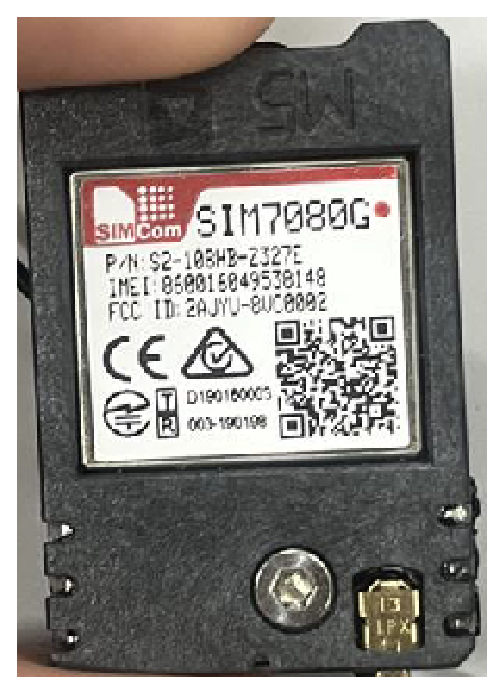
\includegraphics[width=\linewidth]{./figures/porttype}
  \captionof{figure}{SIM7080G}
  \label{fig:SIM7080G}
\end{minipage}
\hfill
\begin{minipage}{0.52\linewidth}
  \centering
  \captionof{table}{SIM7080Gの主なパラメータ}
  \label{tab:sim7080gParameters}
  \begin{tabular}{|c|c|}
    \hline
    項目 & 内容 \\ \hline \hline
    対応通信方式 & LTE Cat.M1 / NB-IoT \\ \hline
    対応周波数帯 & LTE Band 1, 3, 8, 18, 19, 26 ほか \\ \hline
    通信プロトコル & TCP/IP, UDP, HTTP \\ \hline
    動作電圧 & 3.3$\sim$4.2 V \\ \hline
    消費電力(待機時) & 数 mA 程度 \\ \hline
    動作温度範囲 & -40$\sim$85 ℃ \\ \hline
    用途 & M2M / IoT 通信 \\ \hline
  \end{tabular}
\end{minipage}

\end{figure}
\FloatBarrier

\subsection{SIMカード}
本研究では,LTE 通信に IIJ(インターネットイニシアティブ)社が提供する SIM カードを使用した。
本 SIM カードを用いることで,SIM7080G を介したモバイル通信が可能となる。
これにより,設置場所に依存しないデータ収集が可能となり,携帯型測定デバイスとしての有効性を検証できる構成とした。

\section{先行研究で使用した機器}
本研究では,提案手法の有効性を検証するため,先行研究で使用された機器との比較を行った。
本節では,先行研究で用いられた主な機器について説明する。

\subsection{Arduino MKR WiFi 1010}
Arduino MKR WiFi 1010 は,SAMD21G18A マイクロコントローラを中心に,無線通信機能を担う NINA-W102 モジュールや,セキュア通信を実現する暗号チップ ATECC508 を搭載した小型開発ボードである。また,外部 SPI フラッシュメモリとして 2\,MB の記憶領域を備えており,プログラムやデータの保存が可能である。先行研究では,室内環境計測用デバイスの制御用マイクロコントローラとして使用されていた。

\begin{figure}[h]
\centering
\includegraphics[width=.5\linewidth]{./figures/Arduino}
\caption{Arduino MKR WiFi 1010}
\label{fig:Arduino}
\end{figure}
\FloatBarrier

\subsection{CO$_2$センサ MH-Z19C}
MH-Z19C は,Winsen 社が製造する NDIR 方式の CO$_2$ センサモジュールである。比較的安価であり,室内環境測定用途として広く利用されている。先行研究では,本センサを用いて CO$_2$ 濃度の測定が行われていた。本モジュールの主なパラメータを表\ref{tab:mhz19cParameters}に示す。

\begin{figure}[H]
\centering

\begin{minipage}{0.42\linewidth}
  \centering
  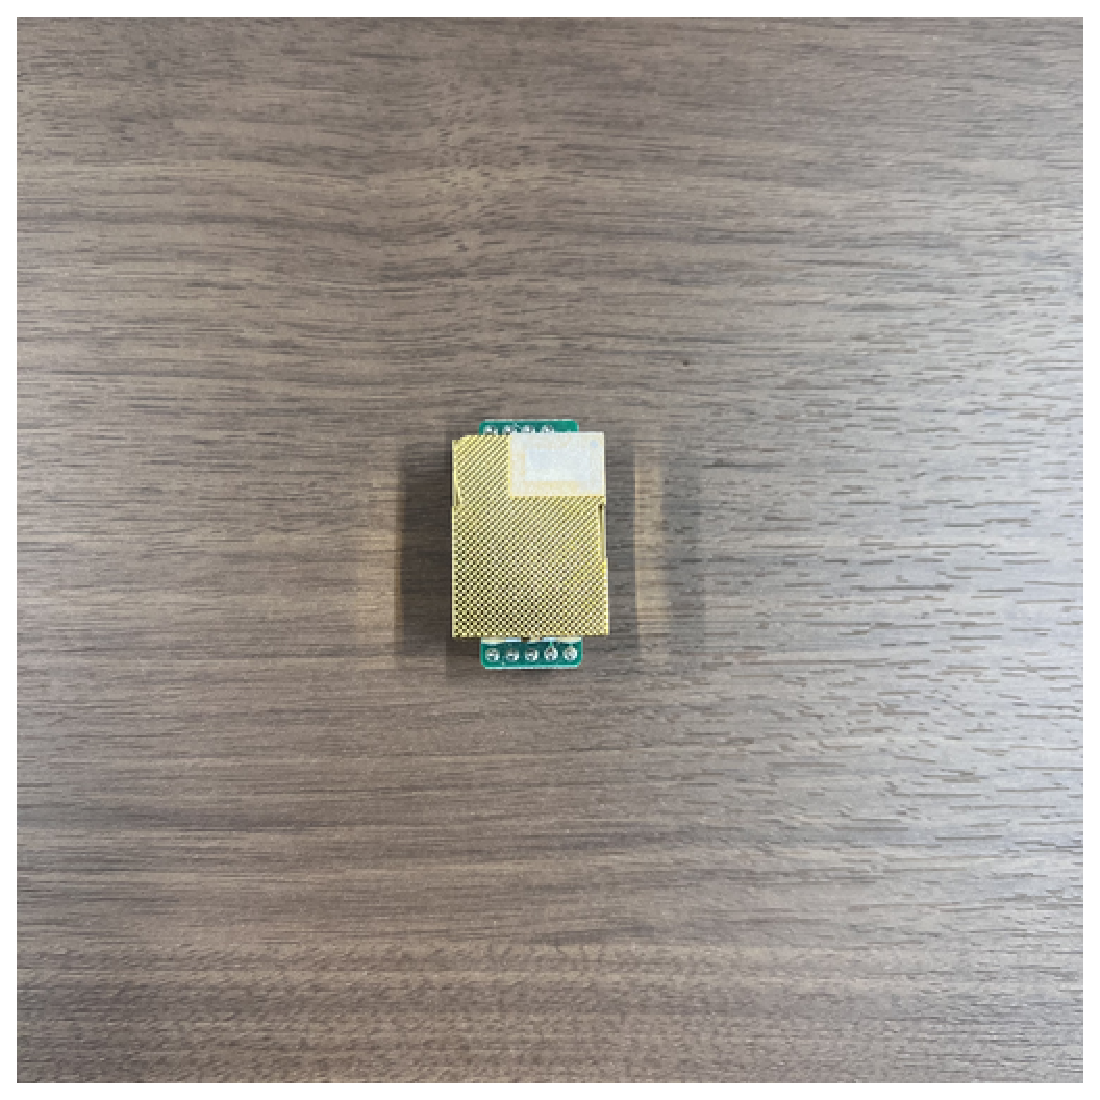
\includegraphics[width=\linewidth]{./figures/mh-z19c}
  \captionof{figure}{MH-Z19C}
  \label{fig:mh-z19c}
\end{minipage}
\hfill
\begin{minipage}{0.52\linewidth}
  \centering
  \captionof{table}{MH-Z19Cの主なパラメータ}
  \label{tab:mhz19cParameters}
  \begin{tabular}{|c|c|}
    \hline
    項目 & 内容 \\ \hline \hline
    測定方式 & NDIR \\ \hline
    CO$_2$測定範囲 & 0$\sim$5000 ppm \\ \hline
    測定精度 & $\pm$(50 ppm + 5\%) \\ \hline
    応答時間 & $<$120 s \\ \hline
    動作電圧 & 4.5$\sim$5.5 V \\ \hline
    平均消費電流 & 約60 mA \\ \hline
    通信方式 & UART / PWM \\ \hline
    用途 & 室内据え置き測定 \\ \hline
  \end{tabular}
\end{minipage}

\end{figure}
\FloatBarrier


\subsection{温度・湿度・気圧センサ BME680}
BME680 は,Bosch Sensortec 社製の環境センサであり,温度,湿度,気圧に加えてガスセンサを内蔵している。内蔵されたガスセンサは主に揮発性有機化合物(VOC)に反応し,室内空気中の汚染度を間接的に評価することが可能である。先行研究では,これら複数の環境指標を組み合わせることで,室内環境を総合的に評価する目的で本センサが使用されていた。本モジュールの主なパラメータを表\ref{tab:bme680Parameters}に示す。

\begin{figure}[H]
\centering

\begin{minipage}{0.42\linewidth}
  \centering
  \includegraphics[width=\linewidth]{./figures/bme}
  \captionof{figure}{BME680}
  \label{fig:BME680}
\end{minipage}
\hfill
\begin{minipage}{0.52\linewidth}
  \centering
  \captionof{table}{BME680の主なパラメータ}
  \label{tab:bme680Parameters}
  \begin{tabular}{|c|c|}
    \hline
    項目 & 内容 \\ \hline \hline
    測定対象 & 温度・湿度・気圧・VOC \\ \hline
    通信方式 & I$^2$C / SPI \\ \hline
    動作電圧 & 1.7$\sim$3.6 V \\ \hline
    用途 & 環境モニタリング \\ \hline
  \end{tabular}
\end{minipage}

\end{figure}
\FloatBarrier

\section{開発環境}
本研究におけるソフトウェア開発には Arduino IDE を使用した。Arduino IDE は,マイクロコントローラ向けの統合開発環境であり,プログラムの作成,コンパイル,書き込みを一貫して行うことができる。本研究では Arduino IDE Version 2.3.7 を使用し,ESP32-C6 および各種センサ,通信モジュールの制御プログラムを開発した。また,Arduino CLI Version 1.3.1 が内部的に用いられており,ビルドおよび書き込み処理が行われている。


%%%%%%%%%%%%%%%%%%%%%%%%%%%%%%%%%%%%%%%%%%%%%%
\chapter{設計}\label{chap:requirement}
% 要求仕様

\section{概要}
本章では,本研究で開発する小型 CO$_2$ 測定デバイスの仕様設計について述べる。
本研究の目的は,携帯可能でありながら高精度な CO$_2$ 濃度測定を可能とするデバイスを
試作し,日常生活のさまざまな環境における換気状況を把握できる仕組みを構築することである。
そのため,本デバイスには小型化,省電力化,測定精度,通信機能といった複数の要件が求められる。


%%%%%

\section{設計仕様}
本研究で開発する CO$_2$ 測定デバイスは,以下の仕様を満たすことを目標とする。

\begin{enumerate}
  \item 測定値と実際の CO$_2$ 濃度との差が小さいこと
  \item 様々な環境において CO$_2$ 濃度を測定できること
  \item 屋外環境を含む様々な場所で長時間利用できること
  \item 小型で持ち運び可能であること
  \item 測定した CO$_2$ 濃度を一定時間おきにサーバへアップロードできること
\end{enumerate}
\vskip1cm

仕様1では,測定値が実際の CO$_2$ 濃度を正確に反映していることを重視する。そのため,経済産業省および産業用ガス検知警報器工業会により制定された「二酸化炭素濃度測定器の選定等に関するガイドライン」を参考にする。同ガイドラインでは,適切な CO$_2$ 濃度測定器の条件として,検知原理に光学式(NDIR 方式など)を用いていること,補正用の機能が測定器に付帯していることが示されている。また,屋外環境において測定を行った際に,測定値が外気中の CO$_2$ 濃度(415~450 ppm 程度)に近い値を示すことや,測定器に呼気を吹きかけた際に CO$_2$ 濃度が大きく上昇すること,さらに,消毒用アルコールを塗布した手や布を測定器に近づけてもCO$_2$ 濃度の測定値が大きく変化しないことが求められている。本研究では,これらの条件に準拠した測定デバイスを設計・開発する。

仕様2では,据え置き型の CO$_2$ 測定器にはない特長として,利用者が移動しながら使用できる点を重視する。自宅や大学,研究室といった固定的な環境に加え,車内や飲食店など多様な環境においても問題なく測定できることを目標とし,携帯型測定デバイスとしての有効性を検証する。

仕様3および仕様4では,携帯型 CO$_2$ 測定デバイスとして屋外環境を含む様々な場所で長時間利用できることを重視する。そのため,商用電源や大型のモバイルバッテリに依存しない構成とし,小型のリチウムポリマーバッテリによる駆動を採用した。また,限られたバッテリ容量で長時間動作を実現するため,デバイス全体の省電力化を図るとともに,筐体の小型化を行った。これにより,ネックレスや腰にぶら下げて持ち運ぶことが可能となり,日常生活の中で手軽に使用できる測定デバイスの実現を目指す。

仕様5では,測定した CO$_2$ 濃度を一定時間間隔でサーバへアップロードする機能を持たせる。


%%%%%




%%%%%%%%%%%%%%%%%%%%%%%%%%%%%%%%%%%%%%%%%%%%%%

\chapter{測定機器の開発}\label{chap:hardwareDevelopment}
% 測定機器実装



\section{測定機器の実装}
本研究では,九電工とも話し合いをしながら,要件仕様を満たす測定機器の開発を行った.  
作成した測定機器は以下の通りである.



%%%%%%%%%%%%%%%%%%%%%%%%%%%%%%%%%%%%%%%%%%%%%%
%\chapter{測定値閲覧機能の開発}\label{chap:softwareDevelopment}
%


本章では,Webシステムにおける測定値閲覧機能について説明する.
本研究室で稼働しているサーバにはWebシステムが設置されており,URLを通じてアクセスすることができる.
測定値閲覧機能は,測定機器の種類や閲覧するデータの内容によって異なるため,複数のシステムが作成されている.
基本的な構成としては,測定機器で測定された値の一覧と測定時間をカラムに持つ表形式と,測定値を可視化したチャート形式の2種類の表示方法を採用している.
チャートの描画には,JavaScriptのフレームワークであるChart.jsを使用している.
以下では,各Webシステムの詳細について述べる.

\section{Arduino用測定値閲覧機能}
Arduino用測定値閲覧機能を,図\ref{fig:ArduinoAirflowChart},図\ref{fig:nowAirflowData}に示す.
データベースに保存された測定値はPHPで取得され,そのデータがJavaScriptにJSON形式で渡されており,
表形式とチャート形式の両方で測定値を表示することができる.
チャートには風速の最大値が表示されている.
更新頻度は約10秒で,最新のデータが取得される仕組みとなっている.


\begin{figure}[h]
\centering
\begin{minipage}{0.49\linewidth}
    \centering
    \includegraphics[width=\linewidth]{./figures/ArduinoAirflowChart}
    \caption{Arduino Airflow Chart}
    \label{fig:ArduinoAirflowChart}
\end{minipage}
\begin{minipage}{0.49\linewidth}
    \centering
    \includegraphics[width=\linewidth]{./figures/nowAirflowData}
    \caption{Now Airflow Data}
    \label{fig:nowAirflowData}
\end{minipage}
\end{figure}

\section{ESP32C6用測定値閲覧機能}
ESP32C6用測定値閲覧機能を,図\ref{fig:webAirGraph},図\ref{fig:webAirTb}に示す.
このWebシステムでは全ての測定値にチャートを対応させた.
チャートの左にある項目から各測定値に表示を切り替えることができる.
更新頻度は約20秒で,表とチャートには100件分の最新データが取得される仕組みとなっている.

\begin{figure}[h]
\centering
\begin{minipage}{0.49\linewidth}
    \centering
    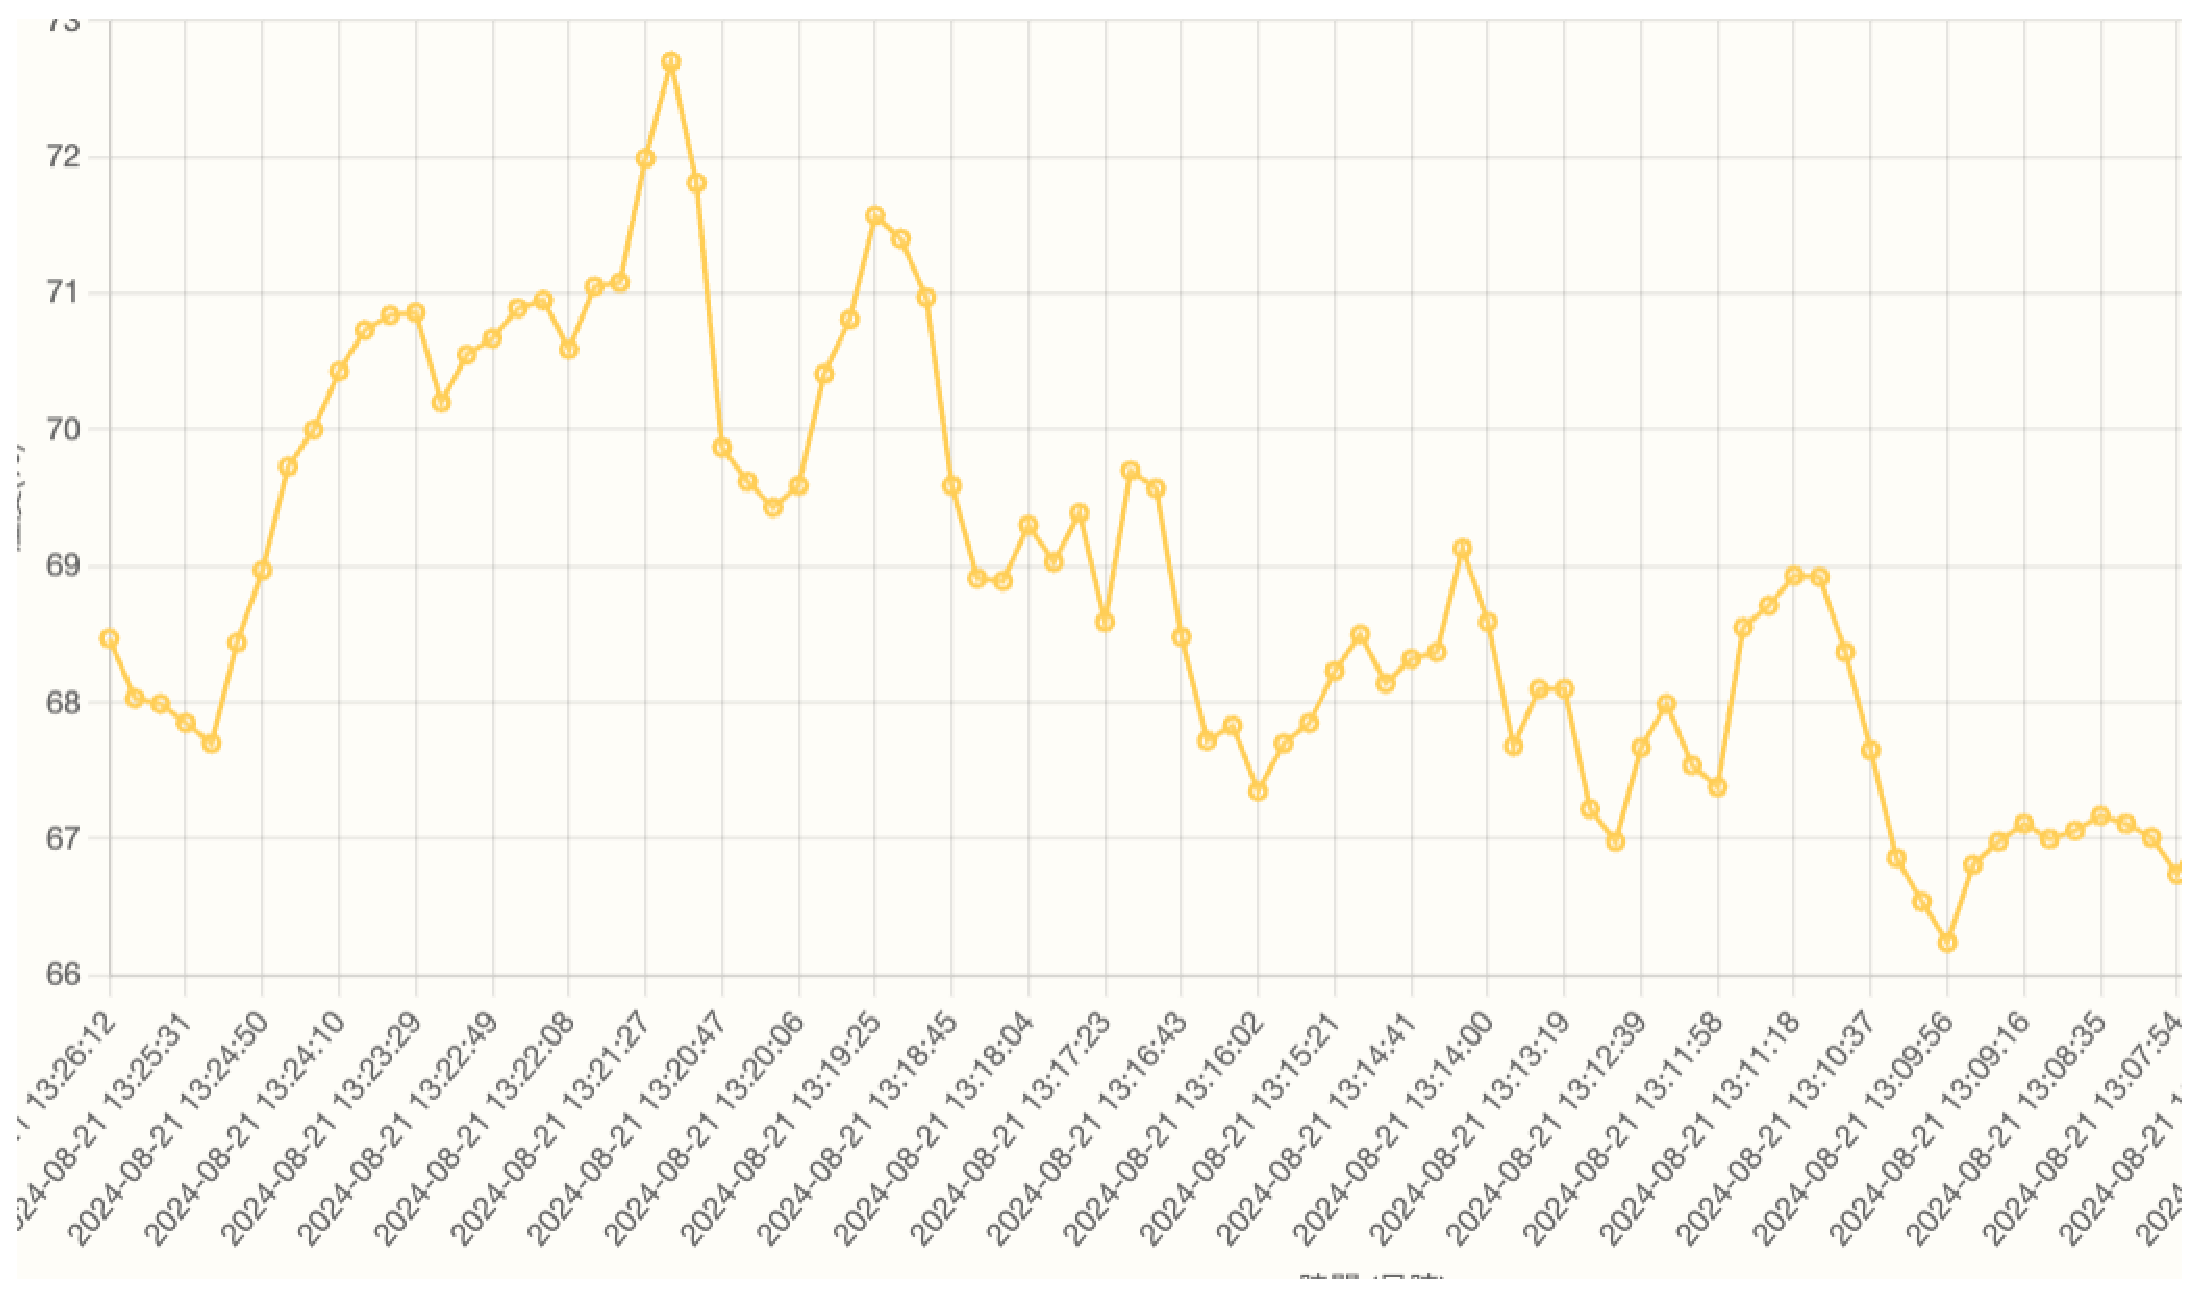
\includegraphics[width=\linewidth]{./figures/webAirTb.eps}
    \caption{測定を表示するグラフ}
    \label{fig:webAirGraph}
\end{minipage}
\begin{minipage}{0.49\linewidth}
    \centering
    \includegraphics[width=\linewidth]{./figures/airTabTable.eps}
    \caption{過去100件の実測値を表示する表}
    \label{fig:webAirTb}
\end{minipage}
\end{figure}




\section{同時に全項目を表示}
同時に全項目を表示する機能を図\ref{fig:airflowCharts}に示す.
このWebシステムは上の項のWebシステムの仕様を変更したバージョンで,同時に一つの項目しか見れなかったものを全ての測定値の項目を一度に見れるようにしたものである.
仮に測定値の項目が増減しても自動で項目も増減し対応する.
更新頻度などは同じ仕様で設計している.

\begin{figure}
\centering
\includegraphics[width=1\linewidth]{./figures/airflowCharts}
\caption{airflowCharts}
\label{fig:airflowCharts}
\end{figure}



\section{デバイスごとの測定値を表示}
デバイスごとの測定値を表示する機能を図\ref{fig:WebSystemESPDeviceIds}に示す.
このWebシステムはこれまで全てのデバイスの測定値を一見の測定値として扱っていたものをデバイスごとに表示する目的で作成した.
ドロップダウンリストでデバイスを選択できること以外仕様は同じ.



\begin{figure}
\centering
\includegraphics[width=1\linewidth]{./figures/WebSystemESPDeviceIds}
\caption{測定機器ごとの測定値を表示するグラフ}
\label{fig:WebSystemESPDeviceIds}
\end{figure}

\section{デバイスをグループ分けして表示}
デバイスをグループ分けして表示する機能を図\ref{fig:ESPGroupGraph}に示す.
このWebシステムはデバイスをグループ分けしてグループごとにグラフを出せるようにしたもの.
専用のページからグループを作成し,デバイスをグループ分けをすることでWebシステムに追加される.
このWebシステムは過去1時間のデータを取得し,20秒ごとに情報を更新する.

\begin{figure}
\centering
\includegraphics[width=1\linewidth]{./figures/ESPGroupGraph}
\caption{グループごとの測定値を表示するグラフ}
\label{fig:ESPGroupGraph}
\end{figure}




\section{冷暖房能力の閲覧機能}

本項では,冷暖房能力の閲覧機能について図\ref{fig:CoolingCapability}に示す.
本機能は空調機器の性能を評価し,表示するために開発を行った.
空調機の冷暖房能力を計算し,その結果をリアルタイムで表示することができる.
このシステムは吹出口の風速,温度,湿度,および吸込口の温度を元に顕熱および潜熱を計算し,
その合計を全熱とし,空調設備の冷暖房能力を表示する.
空調能力に関しては,空調のモデルによって異なるため,モデルに合わせた計算式を使用している.
今回は,本研究室に設置されている\textbf{PLFY-P112EMC6}のモデルに合わせた計算式を使用している.


\subsection*{計算式}

\subsubsection*{顕熱}
顕熱は以下の式で計算する.
\[
Q = V \times \rho \times c \times \Delta T
\]

各項の定義を以下に示す.
\begin{align*}
\rho &= 1.2\,\mathrm{kg/m^3} & \text{(空気密度)} \\
c &= 1.006\,\mathrm{kJ/(kg \cdot K)} & \text{(空気の定圧比熱)} \\
V &= \text{風量(変換後の}\,\mathrm{m^3/s}\text{)} \\
\Delta T &= \text{吸込口と吹出口の温度差}
\end{align*}

\subsubsection*{潜熱}
潜熱も以下の式で計算する.
\[
Q' = V \times \rho \times \Delta h
\]

\subsubsection*{全熱}
 \[
Q_{\text{total}} = Q + Q' = \left( V \times \rho \times c_a \times \Delta T \right) + \left( V \times \rho \times \Delta h \right)
\]


ここで,\(\Delta h\)は比エンタルピーの差を表し,以下の関係で求める.
\[
\Delta h = h_2 - h_1
\]

\begin{align*}
h_1 &= c_a \cdot t_1 + x_1 \cdot (\gamma_o + c_w \cdot t_1) & \text{(吸込口の比エンタルピー)} \\
h_2 &= c_a \cdot t_2 + x_2 \cdot (\gamma_o + c_w \cdot t_2) & \text{(吹出口の比エンタルピー)}
\end{align*}

各項の定義は以下の通りである.
\begin{align*}
t_1 &= \text{吸込口温度(}\mathrm{^\circ C}\text{)}, &
t_2 &= \text{吹出口温度(}\mathrm{^\circ C}\text{)}, \\
x_1 &= \text{吸込口の絶対湿度(}\mathrm{kg/kg(DA)}\text{)}, &
x_2 &= \text{吹出口の絶対湿度(}\mathrm{kg/kg(DA)}\text{)}.
\end{align*}

以下の定数を用いる.
\begin{align*}
c_a &= 1.006\,\mathrm{kJ/(kg(DA) \cdot K)} & \text{(乾き空気の定圧比熱)}, \\
c_w &= 1.805\,\mathrm{kJ/(kg(DA) \cdot K)} & \text{(水蒸気の定圧比熱)}, \\
\gamma_o &= 2501\,\mathrm{kJ/kg} & \text{(水の蒸発潜熱)}.
\end{align*}

\begin{figure}[h]
\centering
\includegraphics[width=1\linewidth]{./figures/CoolingCapability}
\caption{冷暖房能力の閲覧機能}
\label{fig:CoolingCapability}
\end{figure}





%%%%%%%%%%%%%%%%%%%%%%%%%%%%%%%%%%%%%%%%%%%%%%
\chapter{測定方法と評価方法}\label{chap:measurementMethod}
% 評価方法

\section{概要}

本章では,本研究で試作した小型 CO$_2$ 測定デバイスを用い,従来の据え置き型 CO$_2$ センサと比較して,同一環境において同様の CO$_2$ 濃度変化が得られるかを評価する。また,測定デバイスを携帯した状態で,様々な環境において問題なく CO$_2$ 濃度を測定できるかを検証する。はじめに,福岡県赤村に設置されているドームハウス内において,従来の据え置き型 CO$_2$ センサを 35 台設置し,それぞれの近傍に本研究で試作した小型 CO$_2$ 測定デバイスを配置した。この環境において両者の測定値を比較し,CO$_2$ 濃度の時間変化が同様の傾向を示すかを確認した。次に,携帯型デバイスとしての有効性を評価するため,測定デバイスを首の前,首の後ろ,腰の前,腰の後ろの計 4 箇所に装着し,赤村周辺の山道を登る測定を行った。この測定では,装着位置や移動によってCO$_2$ 濃度に異常な変動が生じないかを確認した。
以下では,各測定環境および測定方法について詳述する。

\section{測定環境}
  \subsection{赤村ドームハウス}
  赤村のドームハウスは,複数人が滞在可能な閉鎖空間であり,換気状態や人の滞在による CO$_2$ 濃度変化を評価するのに適した環境である。本測定では,ドームハウス内に従来の据え置き型 CO$_2$ センサを 35 台設置し,それぞれの近傍に小型 CO$_2$ 測定デバイスを配置した。
  
  \subsection{山道における携帯測定環境}
山道における携帯測定は,福岡県赤村に位置する岩石山において実施した。岩石山は標高約 454 m の山であり,登山道が整備されたハイキングコースを有している。本測定では,屋外の移動環境において小型 CO$_2$ 測定デバイスを携帯した状態での測定が可能であるかを評価することを目的とした。測定は登山中に実施し,小型 CO$_2$ 測定デバイスを首の前,首の後ろ,腰の前,腰の後ろの計 4 箇所に装着した。これにより,装着位置や身体の動きによってCO$_2$ 濃度の測定値に異常な変動が生じないかを確認した。

\section{測定方法}
 \subsection{据え置き型センサとの比較測定}

本測定では,据え置き型 CO$_2$ 測定器を複数台設置することで得られる室内の CO$_2$ 濃度分布を基準とし,携帯型の小型 CO$_2$ 測定デバイスが換気状態の把握という目的に対してどの程度有効であるかを評価することを目的とした。そのため,小型測定デバイスを据え置き型測定器の設置位置ごとに順次配置し,同一高さ・同一環境における測定値の比較を行った。

比較測定は,福岡県赤村のドームハウス内に設置された据え置き型 CO$_2$ 測定器を対象として実施した。本測定では,据え置き型 CO$_2$ 測定器を合計 35 台使用し,これらは螺旋階段および 2 階部分に設置された棚を含め,床面付近から天井付近までの高さ方向に配置されている。各測定器には EXAKA1 から EXAKA35 の識別子を付与し,EXAKA1 を最下部,EXAKA35 を最上部とした。

比較測定の手順として,小型 CO$_2$ 測定デバイスを各据え置き型測定器の直近に配置して測定を行い,測定終了後に設置位置を一段上へ移動させる操作を繰り返した。この操作を EXAKA1 から EXAKA35 までの全ての据え置き型測定器に対して順に実施し,合計 35 箇所における比較測定を行った。測定時の小型 CO$_2$ 測定デバイスと据え置き型 CO$_2$ 測定器の配置関係を図\ref{fig:portable_vs_fixed} に示す。本図に示すように,小型測定デバイスは各据え置き型測定器の近傍に設置されており,同一高さ・同一空間におけるCO$_2$ 濃度を測定できるよう配慮した。


  \subsection{携帯時の測定方法}
 本測定では 、図〜に示すように

\section{測定条件}
  \subsection{測定間隔}
  \subsection{装着位置}
  \subsection{測定時間}

\section{評価方法}




%%%%%%%%%%%%%%%%%%%%%%%%%%%%%%%%%%%%%%%%%%%%%%
\chapter{測定結果と評価}\label{chap:measurementResults}
% 評価結果


% 消費電力:USBテスタ(AVHzYct-3)を使用して測定し,消費電力を確認.
% 安定性:波形データから安定性を評価し,機器の安定した計測・データ送信の有無を確認.
% 稼働時間:Webシステムにデータが表示されなくなるまでの時間を測定.
% 精度:市販のTesto 405iと比較して,開発した測定機器の精度を確認.
% 寸法:各機器のサイズ比較.
% 価格:各機器のコストパフォーマンスを評価.
% 他社サービスとの比較:他社の製品やサービス(Testo 405i,Wi-Musu,Gill WindObserver 65など)との比較.




\section{概要}

本章では,第5章までに述べた測定方式および試作した小型 CO$_2$ 測定デバイスを用いて実施した各種測定実験の結果を示し,携帯型測定デバイスとしての有効性および実用性について評価を行うことを目的とする.特に,本研究で試作した携帯型 CO$_2$ 測定デバイスが,据え置き型 CO$_2$ 測定機器と比較して,環境中の CO$_2$ 濃度変化を適切に捉えることができるか,また実際の生活環境や移動環境において利用可能であるかに着目して検討を行う.はじめに,実環境における測定に先立ち,測定機器の基礎特性確認を行う.具体的には,CO$_2$ 測定機器の選定ガイドラインに基づき,アルコールおよび呼気に対する応答特性を評価し,本研究で使用した測定デバイスが CO$_2$ 濃度測定を目的とした機器として適切な特性を有しているかを確認する.この結果を踏まえ,以降の実環境測定において本測定デバイスを用いる妥当性を示す.次に,据え置き型 CO$_2$ 測定機器との比較測定を行い,両者を同一環境下に設置した際の CO$_2$ 濃度の時間変化を比較する.長時間にわたる測定結果を基に,携帯型測定デバイスが据え置き型測定機器と同様の CO$_2$ 濃度変化の傾向を捉えられているかを評価し,携帯型デバイスとしての測定信頼性について検討する.
さらに,空間的に CO$_2$ 濃度のばらつきが生じる環境として,福岡県赤村に設置されたドームハウスを対象に測定を行う.ドームハウス内には,床付近から天井付近にかけて多数の据え置き型 CO$_2$ 測定機器を設置し,高さ方向における CO$_2$ 濃度分布を把握する.その上で,携帯型 CO$_2$ 測定デバイスを用いた測定結果と比較し,空間内における相対的な CO$_2$ 濃度分布や換気が不十分な領域を,携帯型デバイス単体で把握できるかを評価する.
また,実際の生活環境および移動環境における測定例として,電車内における CO$_2$ 濃度の時間変化を測定する.異なる位置において測定を行うことで,車内における換気状況や混雑状況の変化が CO$_2$ 濃度に与える影響を明らかにし,携帯型測定デバイスが移動環境においても有効に機能するかを検討する.
加えて,本章では測定機器の省電力性能および小型化に関する評価を行う.通信方式の異なる測定機器を用いて,バッテリ駆動時の稼働時間を比較することで,通信方式が消費電力に与える影響を明らかにする.また,段階的に試作した測定機器1~4の外形寸法を整理し,小型化の進展について定量的に評価することで,携帯型 CO$_2$ 測定デバイスとしての実用性を検討する.
以上の評価を通じて,本研究で提案する携帯型 CO$_2$ 測定デバイスが,据え置き型測定機器と同様に CO$_2$ 濃度変化を把握可能であり,かつ日常生活環境や移動環境において利用可能な測定手段であることを示す.以下では,各測定環境における測定結果および評価について,順に詳述する.

\subsection{測定機器の基礎特性確認結果および評価}

図\ref{fig:alcohol_breath}に,アルコールおよび呼気に対するCO$_2$濃度の測定結果を示す.測定開始から20分後に,アルコールを入れたコップおよびアルコールを浸したティッシュを測定デバイス近傍に設置したが,この期間においてCO$_2$濃度に顕著な変化は認められなかった.

一方,測定開始から40分後に,測定デバイスに向けて1分間連続して呼気を吹きかけた際には,CO$_2$濃度が急激に上昇する挙動が確認された.この上昇は呼気付与の直後に生じており,呼気中に含まれるCO$_2$に対して測定デバイスが応答していることを示している.

以上の結果から,本研究で使用したCO$_2$測定デバイスは,アルコール蒸気に対しては反応せず,呼気中のCO$_2$に対しては明確に反応する挙動を示した.この挙動は,CO$_2$測定機器の選定ガイドラインに示される基本的な応答特性と整合しており,本デバイスがCO$_2$濃度測定を目的とした測定機器として適切な特性を有していることが確認できる.したがって,本研究では以降の実環境測定において,本測定デバイスを用いてCO$_2$濃度の測定を行うこととした.

\begin{figure}[H]
\centering
\includegraphics[width=0.9\linewidth]{./figures/alcohol}
\caption{
アルコール,呼気への反応結果
}
\label{fig:alcohol_breath}
\end{figure}

\section{据え置き型測定機器との測定値比較}

本節では,据え置き型CO$_2$測定機器と,本研究で試作した携帯型CO$_2$測定デバイスを同一環境下に設置し,両者の測定値の時間変化を比較した結果について述べる.測定は13時30分から24時30分までの約11時間にわたり実施し,両測定機器ともに5分間隔でCO$_2$濃度を測定した.

図\ref{fig:fixed_vs_portable}に,据え置き型測定機器および携帯型測定機器によるCO$_2$濃度の時間変化を示す.測定開始直後には,両測定機器ともに高いCO$_2$濃度を示しており,その後,時間の経過とともにCO$_2$濃度が低下する傾向が確認された.なお,測定開始直後に観測された高いCO$_2$濃度は,測定機器設置作業時に呼気が測定機器近傍にかかったことによる一時的な影響であると考えられる.この低下傾向は,両測定機器においてほぼ同時に観測されている.また,18時30分頃には,両測定機器の測定値においてCO$_2$濃度の上昇が確認され,その後再び低下する挙動が見られた.このようなCO$_2$濃度の増減のタイミングは,据え置き型測定機器と携帯型測定機器の間で概ね一致しており,両者が同一環境におけるCO$_2$濃度変化を捉えていることが分かる.

一方で,携帯型測定機器の測定値は,据え置き型測定機器と比較して一部の時間帯においてわずかな差が見られる.これは,測定機器の設置位置や個体差,応答特性の違いによる影響であると考えられる.しかしながら,CO$_2$濃度の上昇および低下といった時間変化の傾向は両者で概ね一致している.

以上の結果から,本研究で試作した携帯型CO$_2$測定デバイスは,据え置き型CO$_2$測定機器と同様のCO$_2$濃度変化の傾向を示すことが確認できた.このことから,携帯型測定機器は同一環境下においてCO$_2$濃度の時間的な変化を把握する用途において,据え置き型測定機器と同等の情報を取得可能であると考えられる.

\begin{figure}[H]
\centering
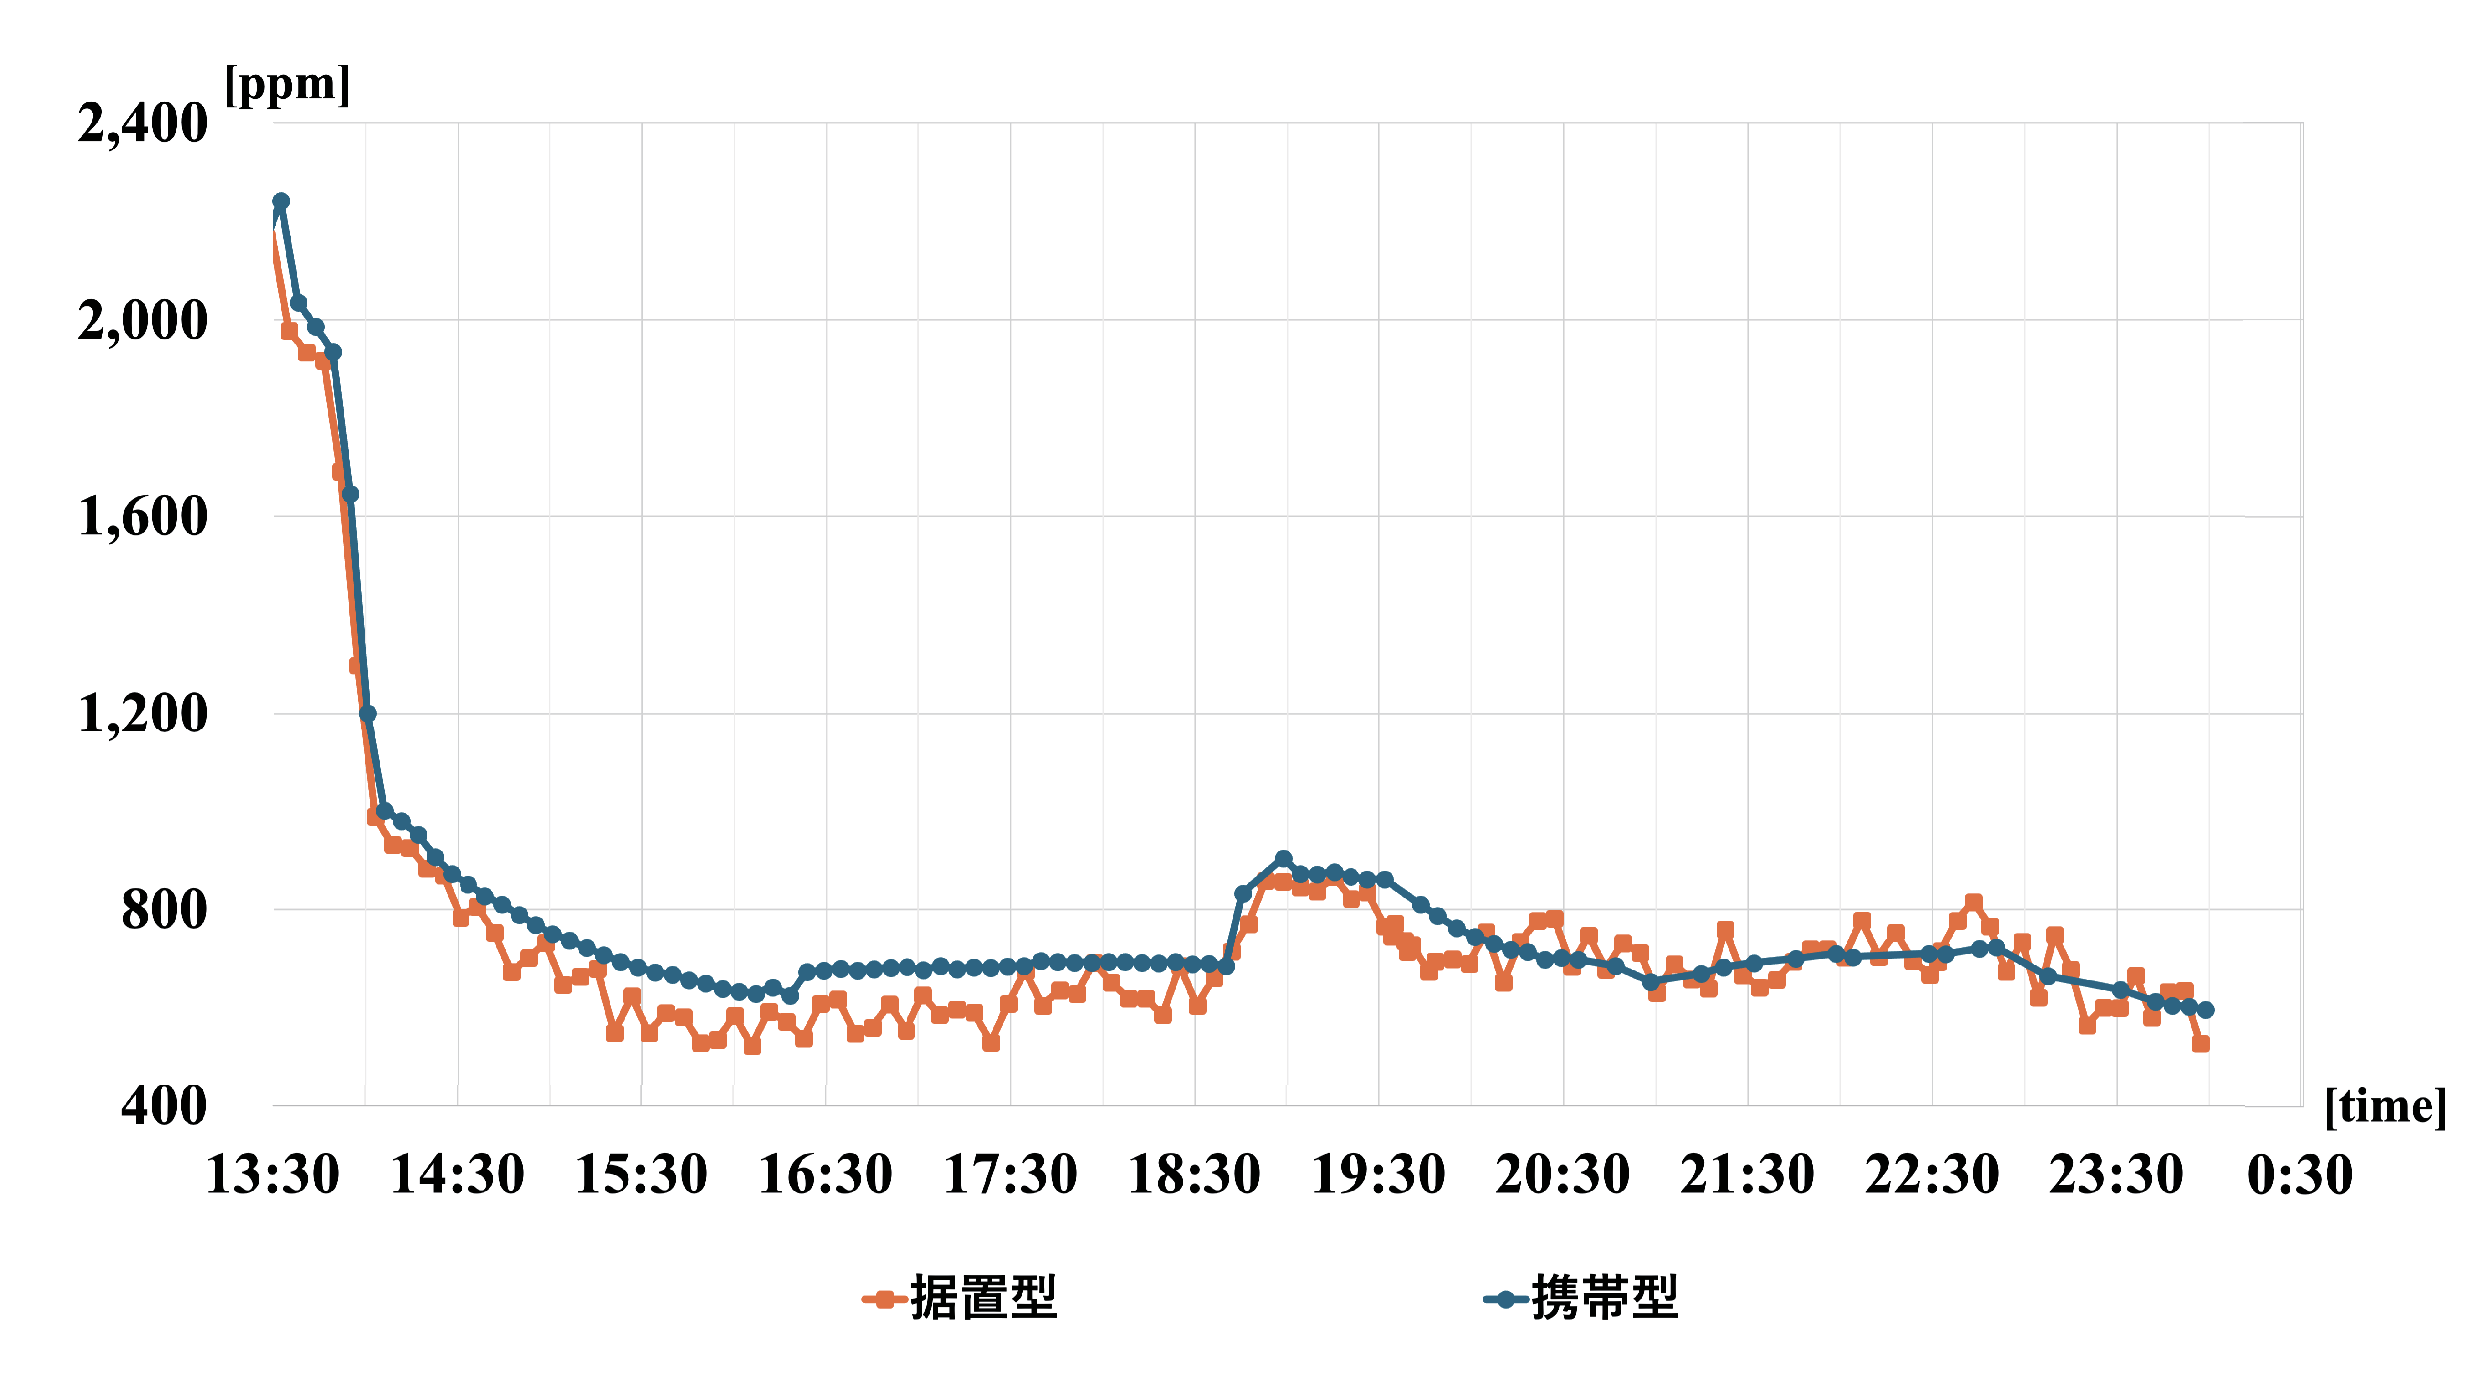
\includegraphics[width=0.9\linewidth]{./figures/センサ比較}
\caption{
据え置き型と携帯型のCO$_2$濃度の比較
}
\label{fig:fixed_vs_portable}
\end{figure}

\section{空間的CO$_2$濃度分布環境における測定結果}
\subsection{ドームハウス内の据え置き型 CO$_2$ 測定機器による測定結果}
据え置き型 CO$_2$ 測定機器を用いてドームハウス内の CO$_2$ 濃度分布を測定した結果を図 \ref{fig:height_co2_comparison} に示す.据え置き型測定機器による測定結果では,階段下から階段上部,さらに 2 階上部へと高さが増加するにつれて,CO$_2$ 濃度が段階的に上昇する傾向が確認された.特に,階段上部および 2 階上部では,階段下部と比較して高い CO$_2$ 濃度が観測されており,ドームハウス内部において CO$_2$ が上部に滞留しやすい空間構造を有していることが示唆される.この結果は,空気の対流や換気経路の影響により,高さ方向に CO$_2$ 濃度の偏りが生じている可能性を示している.


\subsection{ドームハウス内の小型 CO$_2$ 測定デバイスによる測定結果}
次に,本研究で試作した携帯型 CO$_2$ 測定デバイスを用いて,同様にドームハウス内の高さ方向における測定を行った.その結果,小型デバイスにおいても,据え置き型 CO$_2$ 測定機器と同様に,高さの増加に伴って CO$_2$ 濃度が上昇する傾向が確認された.小型デバイスによる測定値は,据え置き型測定機器の測定値と比較して全体的に高い値を示しているが,これはキャリブレーション条件や測定環境の違いによる影響であると考えられる.一方で,階段上部および 2 階上部において CO$_2$ 濃度が高くなるという相対的な変化の傾向は,据え置き型測定機器の結果と概ね一致している.

\subsection{ドームハウス内の据え置き型測定機器との比較評価}

図 \ref{fig:height_co2_comparison} は,据え置き型 CO$_2$ 測定機器および携帯型 CO$_2$ 測定デバイスによる測定結果を,各測定点を 5 点ずつ平均化し,高さ方向に 7 区分して比較したものである.本図より,両者の測定結果は絶対値こそ異なるものの,高さ方向に沿った CO$_2$ 濃度の遷移の仕方が類似していることが分かる.特に,階段下部から階段上部にかけての上昇傾向,および 2 階上部における高濃度領域の検出は,両者で共通して確認された.このことから,小型 CO$_2$ 測定デバイスは,多数の据え置き型測定機器を用いなくても,空間内における CO$_2$ 濃度分布の特徴や,相対的に換気が不十分な領域を把握できる可能性が示された.以上の結果より,本研究で試作した携帯型 CO$_2$ 測定デバイスは,利用者が任意の位置で測定を行うことで,空間内の危険性が高い領域を簡便に察知する手段として有効であると考えられる.

\begin{figure}[H]
\centering
\includegraphics[width=0.9\linewidth]{./figures/赤村比較}
\caption{
各測定点におけるCO$_2$濃度比較
}
\label{fig:height_co2_comparison}
\end{figure}




\section{電車内における CO$_2$ 濃度変化}

本節では,JR 九州 鹿児島本線において実施した電車内測定について,
鳥栖行き普通列車(行き)および門司港行き普通列車(帰り)の
2 つの測定結果を示し,
乗客数の変化,ドア開閉状況,および測定位置の違いが
CO$_2$ 濃度に与える影響について考察する.

\subsection{行き(鳥栖行き普通列車)における測定結果}

行きの測定は,鳥栖行き普通列車において実施した.測定結果を図\ref{fig:densya_iki}にしめす.測定は 1 両目において,進行方向最後部のドア付近に位置し,携帯型 CO$_2$ 測定デバイスを腰部に装着した状態で行った.20 時 32 分に九産大前駅から乗車し,21 時 33 分に鳥栖駅へ到着するまでの区間を対象とした.

測定開始直後(20:32~20:40 頃)は,車内の乗客数が少なく,CO$_2$ 濃度は比較的低い値で推移していた.その後,博多駅(20:47 停車)において多数の乗客が乗車したことにより,発車直後から CO$_2$ 濃度の上昇が確認された.この上昇は,乗客の増加に伴う呼気由来の CO$_2$ 発生量の増加によるものと考えられる.

一方,竹下駅(20:51),笹原駅(20:55),南福岡駅(20:58)以降では,乗客が段階的に降車したことに伴い,CO$_2$ 濃度は徐々に低下する傾向を示した.特に,原田駅(21:17 停車)では,列車の待ち合わせのためドアが長時間開放されており,この区間において CO$_2$ 濃度の顕著な低下が観測された.これは,ドア開放による外気流入が車内換気を大きく促進した結果であると考えられる.

以上より,行きの測定結果からは,乗客数の増減およびドア開閉状況が電車内の CO$_2$ 濃度に直接的な影響を与えることが確認できた.


\begin{figure}[H]
\centering
\includegraphics[width=0.7\linewidth]{./figures/電車比較_行き}
\caption{
電車内のco2濃度変化
}
\label{fig:densya_iki}
\end{figure}



\subsection{帰り(門司港行き普通列車)における測定結果}

帰りの測定は,門司港行き普通列車において実施した.測定結果を図\ref{fig:densya_kaeri}に示す.
測定位置は 9 両目の進行方向先頭側ドア付近とし,21 時 41 分に鳥栖駅から乗車し,22 時 43 分に九産大前駅へ到着するまで測定を行った.乗車時点での車内人数は約 4 名と少なく,発車までの間はドアが開放された状態であった.

測定開始直後は,車内の乗客数が少ないことに加え,ドアが開放されていたため,CO$_2$ 濃度は 500~600 ppm 程度の低い値で安定して推移した.その後,各駅での停車と発進を繰り返す中でも,乗客数の変化が小さい区間ではCO$_2$ 濃度に大きな変動は見られなかった.

一方,博多駅(22:26 停車)では,多くの乗客が乗車したことにより,発車後に CO$_2$ 濃度が急激に上昇する挙動が確認された.さらに,ドア付近で会話を行う乗客が存在した区間では,局所的に CO$_2$ 濃度が高くなる傾向が見られた.その後,香椎駅(22:38 停車)では,乗客の降車およびドア開放が長時間続いたことにより,CO$_2$ 濃度は再び低下した.

このように,帰りの測定結果からは,車内人数が少ない状態ではCO$_2$ 濃度が低く保たれる一方で,主要駅における大量乗車やドア付近での会話といった局所的要因により,短時間で CO$_2$ 濃度が上昇することが確認された.
\begin{figure}[H]
\centering
\includegraphics[width=0.7\linewidth]{./figures/電車比較_帰り}
\caption{
電車内のco2濃度変化
}
\label{fig:densya_kaeri}
\end{figure}
\FloatBarrier

\subsection{ドア付近とドアから離れた位置における CO$_2$ 濃度の比較}

本測定では,電車内における換気状況の位置依存性を評価するため,ドア付近(CS2)およびドアから離れた位置(CS1)の2 箇所において CO$_2$ 濃度の測定を行った.両測定点はいずれも同一車両内に位置しているが,ドア開閉や外気流入の影響の受けやすさが異なる点が特徴である.

行きおよび帰りの測定結果を通して,両測定点の CO$_2$ 濃度は概ね同様の増減傾向を示したものの,濃度の絶対値には明確な差が確認された.特に,多くの時間帯において,ドアから離れた位置(CS1)の CO$_2$ 濃度が,ドア付近(CS2)よりも高くなる傾向が見られた.

例えば,行きの測定においては,博多駅通過後の混雑区間において,CS1 では 1300 ppm を超える値が観測された一方,CS2 ではそれより低い値で推移している.これは,ドア付近では停車時のドア開閉に伴って外気が流入しやすく,局所的な換気が促進されるのに対し,ドアから離れた位置では外気流入の影響を受けにくく,呼気由来の CO$_2$ が滞留しやすいためであると考えられる.

また,各駅停車時に着目すると,
ドア開放直後に CO$_2$ 濃度が低下する挙動は
ドア付近(CS2)でより顕著に現れており,ドアから離れた位置(CS1)では低下量が小さい,あるいは時間遅れを伴って現れる場合があった.この結果は同一車両内であっても換気効果が一様ではなく,位置によって大きく異なることを示している.
以上の結果から,電車内においてはドア付近では比較的換気が行われやすい一方で,ドアから離れた座席付近ではCO$_2$ 濃度が高くなりやすい傾向があることが明らかとなった.本研究で試作した携帯型 CO$_2$ 測定デバイスを用いることで,このような車内の位置による換気状況の違いを利用者自身が把握できる可能性が示された.

\section{省電力性能の評価結果}

本節では,測定機器3および測定機器4において,バッテリ駆動時の稼働時間を測定し,通信方式およびシステム構成の違いが消費電力に与える影響について評価を行う.

先行研究においては,Arduino MKR WiFi 1010,MH-Z19C,BME680,および 1100\,mAh のリチウムポリマバッテリを用いたCO$_2$ 測定機器が試作されており,据え置き型センサを携帯可能とする試みが行われていた.しかし,これらの構成では,Wi-Fi 通信および常時動作に伴う消費電力が大きく,連続稼働時間はおおよそ 6~9 時間程度にとどまることが想定されている.このことから,携帯型 CO$_2$ 測定機器の実用化に向けては,さらなる省電力化が課題であった.


\begin{figure}[H]
\centering
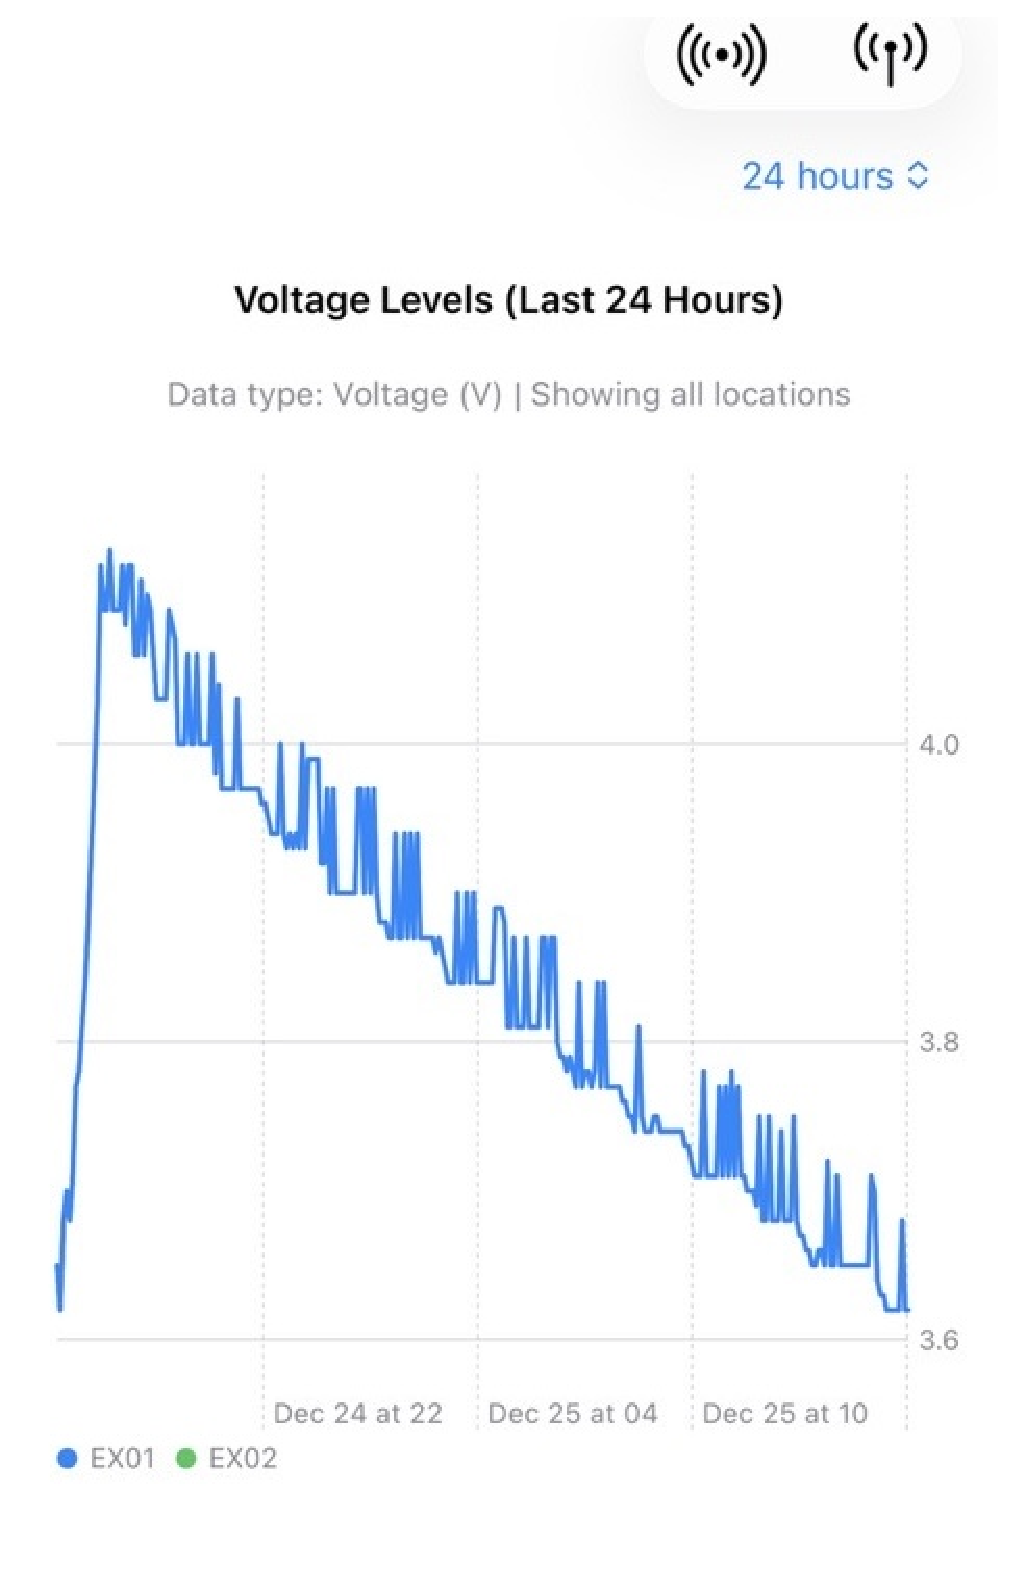
\includegraphics[width=0.5\linewidth]{./figures/voltage-Arduino}
\caption{
測定機器3のバッテリ持続時間
}
\label{fig:voltage-Arduino}
\end{figure}
\FloatBarrier


本研究では,この課題を解決するため,ESP32-C6 を用いたマイクロコントローラ構成と,DeepSleep を活用した周期動作方式を採用し,通信方式の違いによる消費電力の低減効果について検討した.各測定機器には容量 250\,mAh のリチウムポリマバッテリを使用し,測定間隔は 5 分とした.測定時には CO$_2$ 濃度の取得および必要な通信処理を行い,それ以外の時間は ESP32-C6 を DeepSleep 状態へ移行させる構成とした.この条件の下で,バッテリ電圧の時間変化および連続稼働時間を測定した.

LTE 通信モジュール SIM7080G を搭載した測定機器4では,0 時から 15 時までの約 15 時間にわたり連続動作することを確認した.図\ref{fig:voltage} に示すように,動作開始直後は約 4.1\,V 付近であったバッテリ電圧が,時間の経過とともに徐々に低下し,動作終了時には約 3.0\,V まで低下した.この間,設定した測定間隔で測定および通信処理が正常に実行されており,LTE 通信を含む構成においても,DeepSleep を用いた周期動作が実現できていることが確認できた.

\begin{figure}[H]
\centering
\includegraphics[width=0.5\linewidth]{./figures/voltage}
\caption{
測定機器4のバッテリ持続時間
}
\label{fig:voltage}
\end{figure}
\FloatBarrier

一方で,LTE 通信を使用しない測定機器3について評価を行った.測定機器3では,Wi-Fi を用いて測定データを送信する構成であり,LTE 通信モジュールを搭載していない点が特徴である.そのため,セルラ通信に比べて通信時の消費電力を抑えた動作が可能である.その結果,同一条件(測定間隔 5 分,DeepSleep 使用,バッテリ容量 250\,mAh)において,約 56 時間の連続稼働を確認した.

\begin{figure}[H]
\centering
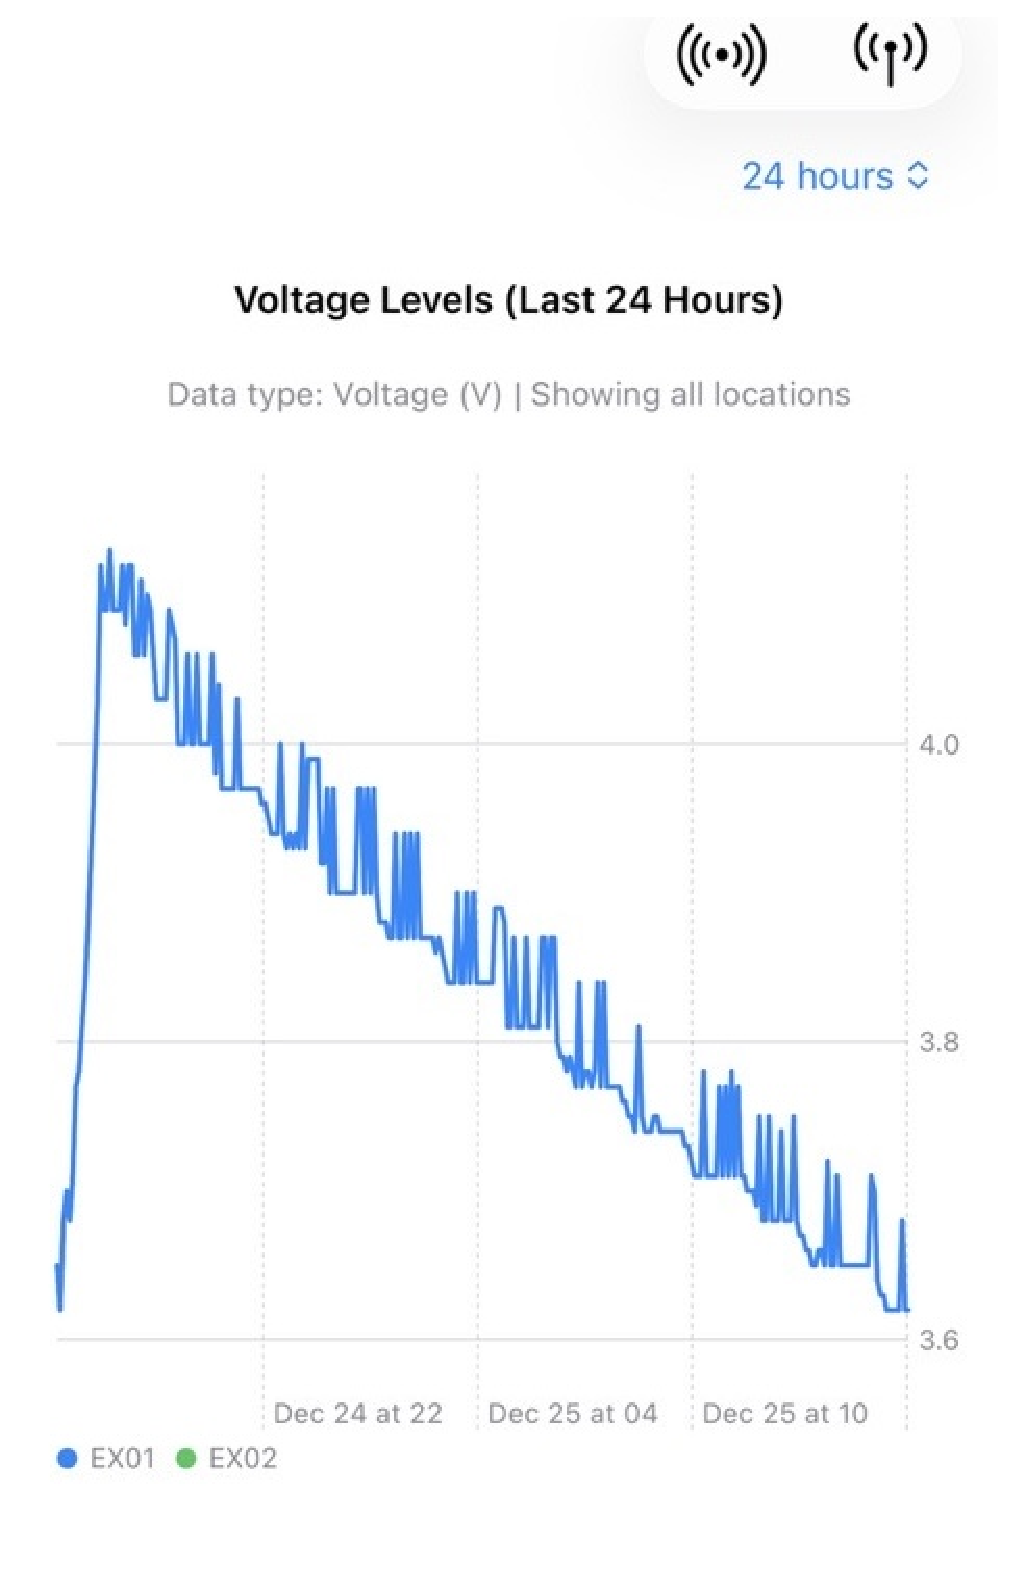
\includegraphics[width=0.5\linewidth]{./figures/voltage-Arduino}
\caption{
測定機器3のバッテリ持続時間
}
\label{fig:voltage-Arduino}
\end{figure}
\FloatBarrier

これらの結果から,先行研究における MH-Z19C を用いた携帯型測定機器と比較して,本研究で提案する測定機器は,バッテリ容量が小さいにもかかわらず,稼働時間を大幅に延長できていることが分かる.特に,Wi-Fi 通信を用いた測定機器3では,先行研究の構成と比較して,約 6 倍以上の連続稼働時間を実現しており,DeepSleep を活用した周期動作設計の有効性が示された.

以上より,本研究で提案する測定機器は,利用目的に応じて通信方式を選択することで,携帯性と稼働時間のバランスを柔軟に調整できる携帯型 CO$_2$ 測定デバイスであることが確認された.


\section{小型化に関する評価}

本節では,本研究で段階的に開発した測定機器1~4について,筐体の小型化の観点から評価を行う.携帯型 CO$_2$ 測定デバイスとして日常生活での利用を想定した場合,測定精度や通信性能に加えて,機器の大きさは携帯性や使用頻度に大きく影響する重要な要素である.

従来,本研究室の先行研究において,据え置き型 CO$_2$ 測定機器が作成され,室内環境における CO$_2$ 濃度の定点観測に用いられてきた.これらの据え置き型測定機器は,長時間にわたる安定した測定が可能であり,空間全体の換気状態を把握する上で有効である一方で,外形寸法が大きく,利用者が身につけて移動しながら測定を行う用途においては,
携帯性の観点から実用が困難であることが,先行研究における課題点として挙げられていた.

そこで本研究では,先行研究で明らかとなった「持ち運びには大きい」という課題を解決することを目的として,小型 CO$_2$ 測定デバイスの開発を行った.
据え置き型測定機器の測定精度や測定手法を踏襲しつつ,日常生活のさまざまな環境において利用者が携帯可能なサイズを実現することを目標とし,小型化を重視した設計を行った.

表\ref{tab:size_comparison}に,据え置き型測定機器および測定機器1~4の外形寸法と体積(外形面積)の比較を示す.据え置き型測定機器は外形寸法が約 73\,mm $\times$ 65\,mm,外形面積が約 4,745\,mm$^2$ であり,携帯型として使用するには大きいことが分かる.これに対し,本研究で試作した測定機器はいずれも,据え置き型測定機器と比較して大幅な小型化が達成されている.

\begin{table}[htbp]
\centering
\caption{据え置き型測定機器および測定機器1~4の外形寸法と体積の比較}
\label{tab:size_comparison}
\begin{tabular}{|l|r|r|}
\hline
測定機器 & 外形寸法 [mm] & 体積 [mm$^2$] \\ \hline \hline
据え置き型測定機器 & 73 $\times$ 65 & 4,745 \\ \hline
測定機器1 & 40 $\times$ 60 & 2,400 \\ \hline
測定機器2 & 50 $\times$ 70 & 3,500 \\ \hline
測定機器3 & 30 $\times$ 40 & 1,200 \\ \hline
測定機器4 & 35 $\times$ 55 & 1,925 \\ \hline
\end{tabular}
\end{table}

測定機器1は,ESP32-C6,SCD41,プッシュボタンおよびリチウムポリマバッテリを用いた最小構成の測定機器であり,外形寸法は約 40\,mm $\times$ 60\,mm であった.本機器は機能確認を主目的として作成したため,部品配置の最適化や筐体サイズの削減は行っておらず,比較的余裕のある寸法となっている.しかしながら,据え置き型測定機器と比較すると,外形面積は約 50\% 程度に抑えられており,携帯型測定機器としての可能性を示す結果である.

測定機器2では,測定機器1の構成を維持したまま,利用者への視覚的フィードバックを目的として LED を追加した.その結果,外形寸法は約 50\,mm $\times$ 70\,mm となり,測定機器1と比較してやや大型化している.これは機能追加を優先した設計によるものであり,試作段階における仕様上の選択である.それでもなお,据え置き型測定機器と比較すると外形面積は小さく,携帯型測定機器としての基本的な要件は満たしている.

測定機器3では,測定機器2で確認された機能を維持しつつ,携帯性の向上を目的として筐体の小型化を行った.部品配置を見直し,ESP32-C6 の表面および裏面の両方に部品を実装する構成とすることで,外形寸法は約 30\,mm $\times$ 40\,mm まで縮小された.測定機器1と比較すると,外形面積は約 2,400\,mm$^2$ から約 1,200\,mm$^2$ へと減少しており,約 50\% の削減が達成されている.また,据え置き型測定機器と比較すると,外形面積は約 75\% 削減されており,本研究の目的である携帯性の向上が大きく達成されたことが分かる.

さらに,測定機器4では,測定機器3で達成した小型化を意識しつつ,LTE 通信モジュールである SIM7080G を新たに搭載した.通信機能の追加により構成は複雑化したものの,外形寸法は約 35\,mm $\times$ 55\,mm に抑えられている.

測定機器2と比較すると,外形面積は約 3,500\,mm$^2$ から約 1,925\,mm$^2$ へと減少しており,約 45\% の小型化が実現されている.これは,通信機能を追加しながらも,部品配置の最適化によって筐体の縮小が可能であったことを示している.また,据え置き型測定機器と比較すると,外形面積は約 4,745\,mm$^2$ から約 1925\,mm$^2$ へと減少しており,約 60\% の小型化が達成されている.この結果から,LTE 通信を備えた構成であっても,据え置き型測定機器では困難であった携帯性を確保できることが明らかとなった.

以上の結果から,本研究では据え置き型 CO$_2$ 測定機器の課題であった大型化という問題に対し,ESP 系マイクロコントローラを用いた段階的な設計改良を行うことで,機能追加と小型化の両立を実現してきたといえる.特に,測定機器3および測定機器4では,,ネックレスや腰部への装着といった利用形態にも適した携帯型 CO$_2$ 測定デバイスであると評価できる.









%%%%%%%%%%%%%%%%%%%%%%%%%%%%%%%%%%%%%%%%%%%%%%
 \chapter{結論}\label{chap:conclusion}
% 結論

\section{まとめ}


\begin{comment}
一つ目は,空調に設置可能で,自動で風速や温湿度を測定できるIoT機器の開発である.
特に,風速については,405iの測定値と比較して誤差を10\%以内に抑えることを目標とし,
さらに1週間の稼働を目指す.
二つ目は,測定機器の測定値を記録し,測定値をリアルタイムで閲覧できるシステムの開発である.
\end{comment}



本研究では,日常生活環境における換気状態の把握を目的として,携帯可能な小型 CO$_2$ 測定デバイスの設計・試作および評価を行った.従来の据え置き型 CO$_2$ 測定器は,設置場所が限定されることや,利用者の周囲環境を直接的に把握することが難しいという課題があった.これに対し,本研究では,利用者が身につけて使用できる携帯型デバイスに着目し,小型化・省電力化・測定精度・通信機能を両立したCO$_2$ 測定システムの実現を目指した.

まず,設計段階においては,経済産業省および産業用ガス検知警報器工業会により制定された「二酸化炭素濃度測定器の選定等に関するガイドライン」を参考とし,CO$_2$ 濃度測定器に求められる基本的な性能を満たすことを重視した.具体的には,呼気中の CO$_2$ に対して適切に応答する一方で,消毒用アルコールなどの揮発性成分に対して誤反応しないこと,および安定した測定が可能であることを設計方針として採用した.これらの指針に基づき,光学式 CO$_2$ センサを中心とした構成を採用し,携帯型デバイスとしての実用性を考慮したシステム設計を行った.

次に,試作した携帯型 CO$_2$ 測定デバイスについて,実環境での測定に先立ち,センサの基礎特性確認を実施した.アルコールおよび呼気に対する応答を評価した結果,アルコールに対しては測定値の大きな変動が見られなかった一方で,呼気を吹きかけた際には CO$_2$ 濃度の顕著な上昇が確認された.この結果から,本研究で使用した CO$_2$ 測定デバイスは,ガイドラインに示される基本的な応答特性を満たしており,実環境における CO$_2$ 濃度測定に適したセンサであることが確認された.

据え置き型 CO$_2$ センサとの比較測定では,同一環境下において両者を設置し,長時間にわたる CO$_2$ 濃度の時間変化を比較した.その結果,測定開始直後に見られた高い CO$_2$ 濃度は,設置時に呼気がセンサにかかった影響であると考えられるものの,その後の時間変化においては,据え置き型センサと携帯型センサが同様の増減傾向を示すことが確認された.一部の時間帯において測定値に差が見られたものの,CO$_2$ 濃度の上昇および低下のタイミングは概ね一致しており,携帯型デバイスが環境中の CO$_2$ 濃度変化を適切に捉えていることが示された.

さらに,赤村ドームハウスにおける測定では,高さ方向に CO$_2$ 濃度の分布が生じる環境において,携帯型デバイスが利用者周囲の CO$_2$ 濃度を把握できるかを検証した.多数の据え置き型センサによる測定結果と比較した結果,携帯型デバイスによる測定値は,設置位置に応じた CO$_2$ 濃度の違いを反映しており,空間内の換気状態を把握する手段として有効であることが確認された.この結果から,携帯型 CO$_2$ 測定デバイスは,空間全体の分布を把握する用途に加え,利用者の周囲環境を評価する用途においても有用であると考えられる.

また,電車内における測定では,公共交通機関という人の乗降や換気条件が刻々と変化する環境において測定を行った.ドア付近およびドアから離れた座席位置において測定した結果,ドア開閉や乗客の乗降に伴う CO$_2$ 濃度の変化が確認され,測定位置による濃度差が生じることが示された.このことから,携帯型 CO$_2$ 測定デバイスは,移動環境においても測定可能であり,公共交通機関内の換気状況や空気環境を評価する手段として活用できる可能性が示唆された.

省電力性能の評価においては,周期的な測定・通信・待機動作を採用することで,バッテリ駆動による長時間動作が可能であることを確認した.これにより,携帯型デバイスとして日常的に使用する際にも,頻繁な充電を必要としない実用的な運用が可能であると考えられる.

以上の結果から,本研究で試作した携帯型 CO$_2$ 測定デバイスは,ガイドラインに基づく基本的な測定性能を満たし,据え置き型センサと同様の CO$_2$ 濃度変化を捉えることができること,ならびに屋内外や移動環境を含むさまざまな実環境において利用可能であることが示された.本研究の成果は,換気状態の可視化や空気環境の把握を目的とした携帯型 CO$_2$ 測定システムの実現に向けた有用な知見を提供するものである.

\section{今後の課題}

本研究により,携帯型 CO$_2$ 測定デバイスの有効性および実環境における測定可能性が示された一方で,実用化および応用展開を見据えた際には,いくつかの課題が残されている.本節では,本研究を通じて明らかになった今後の課題について述べる.

\subsection{稼働時間の向上}

本研究では,通信方式として Wi-Fi および LTE を用いた測定機器を試作し,それぞれの省電力性能について評価を行った.その結果,テザリングや Wi-Fi 環境を利用した ESP32-C6 単体の測定機器においては,周期的な測定および待機動作を採用することで,十分な省電力動作が可能であることが確認された.一方で,LTE 通信を用いた測定機器では,通信時の消費電力が大きく,バッテリ駆動による連続稼働時間が約 16 時間程度にとどまった.

携帯型デバイスとして日常生活の中で継続的に利用することを想定した場合,1 日以上の連続稼働が可能であることが望ましい.そのため,今後は LTE 通信時の消費電力削減を目的として,通信頻度のさらなる最適化や,送信データ量の削減,通信モジュールのスリープ制御の高度化などを検討する必要がある.また,バッテリ容量の見直しや,高効率な電源回路の導入も,稼働時間向上に向けた有効な手段であると考えられる.

\subsection{測定機器のケース作成}

本研究では,測定機器の小型化を重視した設計を行ったものの,現状の試作機ではセンサ部や電子部品が外部に露出しており,持ち運び時や日常使用時における破損の危険性が残されている.また,外部からの衝撃や埃,湿気などの影響を受けやすい構造であることも課題として挙げられる.

一方で,CO$_2$ センサは周囲空気を直接取り込む必要があるため,完全に密閉されたケースを用いることは測定結果に影響を及ぼす可能性がある.そのため,今後は,通気性を確保しつつ,センサおよび回路を保護できるケース構造の検討が必要である.例えば,通気孔の配置やフィルタ材の使用,3D プリンタを用いた専用ケースの設計などが考えられる.これにより,携帯性および耐久性を向上させ,実用的な測定機器としての完成度を高めることが期待される.

\subsection{授業姿勢の判定への応用}

本研究で試作した携帯型 CO$_2$ 測定デバイスは,利用者の周囲環境における CO$_2$ 濃度を直接測定できるという特徴を有している.この特性を応用することで,教室環境における換気状態の把握だけでなく,授業中の姿勢や行動状態の推定への応用が考えられる.

例えば,着席状態で前傾姿勢をとった場合や,顔が机に近づいた場合には,呼気の影響によりセンサ近傍の CO$_2$ 濃度が一時的に上昇する可能性がある.このような CO$_2$ 濃度の変動パターンを,加速度センサや姿勢センサなどの他のセンサ情報と組み合わせることで,授業中の姿勢や集中状態を推定する手法へと発展させることが考えられる.今後は,複数センサを組み合わせたデータ取得および解析手法の検討が課題である.

\subsection{長期間運用における信頼性評価}

本研究では,短期間の測定を中心に評価を行ったが,実用化を見据えた場合,長期間にわたる連続運用時の信頼性評価が重要となる.特に,センサの経時的なドリフトや,環境条件の変化による測定精度への影響については,十分な検証が必要である.

今後は,数日から数週間にわたる連続測定を行い,測定値の安定性や再現性を評価するとともに,必要に応じて補正手法の導入を検討することが求められる.




%%%%%%%%%%%%%%%%%%%%%%%%%%%%%%%%%%%%%%%%%%%%%%

%\chapter*{謝辞}
%\addcontentsline{toc}{chapter}{謝辞}
%本研究の遂行および本論文の執筆にあたり,多大なるご指導とご支援を賜りました九州産業大学理工学部情報科学科の田中康一郎教授に,心より感謝申し上げます.研究の進め方のみならず,問題に対する考え方や研究者としての姿勢についても多くのことをご教示いただきました.日々の議論や助言を通して,研究に対する視野を広げる貴重な機会を与えていただいたことに,深く感謝しております.

また,2 年間にわたり同じ研究室に所属し,ともに研究活動に取り組んだ学部 4 年の青柳貴之氏,上原一眞氏,木村光翔氏,須賀翔一氏,竹内勇人氏,平田健斗氏,嶺田あんず氏には,心から感謝いたします.研究が思うように進まない時期においても,互いに意見を交換し,励まし合いながら研究を進めることができたことは,本研究を完成させる上で大きな支えとなりました.日々の研究活動を通して,多くの刺激を受け,ともに成長できたことを大変嬉しく思います.

さらに,学部 3 年の阿比留新太氏,彌永大翔氏,岡野望生氏,熊添翠杏氏,佐藤乃果氏,島崎佑亮氏,野坂卓矢氏,日高祥平氏には,測定実験やデータ整理など,研究活動のさまざまな場面において多大な協力をいただきました.忙しい中にもかかわらず,快く研究を手伝っていただいたことに,深く感謝いたします.皆様の協力なくして,本研究を円滑に進めることはできませんでした.

最後に,大学 4 年間にわたり,経済的にも精神的にも支えてくれた家族に心から感謝します.研究や学業に集中できる環境を与えてくれたこと,そして常に温かく見守り続けてくれたことに,深く感謝しております.

\begin{flushright}
2026/1

井上誠斗
\end{flushright}\clearpage{}
%%%%%%%%%%%%%%%%%%%%%%%%%%%%%%%%%%%%%%%%%%%%%%
\addcontentsline{toc}{chapter}{参考文献}
\bibliography{paper}
\bibliographystyle{tipsj}
%%%%%%%%%%%%%%%%%%%%%%%%%%%%%%%%%%%%%%%%%%%%%%

%%% 付録 %%%
\appendix\clearpage{}

%\chapter{開発環境}\label{achap:Evaluation}
%\addcontentsline{toc}{chapter}{開発環境}
%\input{7IDE.tex}\clearpage{}

%%%%%%%%%%%%%%%%%%%%%%%%%%%%%%%%%%%%%%%%%%%%%%

%%%%%%%%%%%%%%%%%%%%%%%%%%%%%%%%%%%%%%%%%%%%%%

%\chapter{ソースコード}\label{achap:Evaluation}
%\addcontentsline{toc}{chapter}{ソースコード}
%\input{9cord.tex}\clearpage{}
\end{document}

